\section{统计计算与软件部分}\label{SecStatisticalComputingAndSoftware}
\begin{center}
    Instructor: Zaiying Zhou
\end{center}

\subsection{Algorithm Theory Introduction}

% \subsubsection{Float Storage}

\subsubsection{Finite Precision Computation}
    An arbitrary real number $ r\in\mathbb{R} $ is represented as (the nearest adjacent) float number $ v_r $. A float is basically stored as (example take 32-bit float): 1 bit \textbf{S}ign + 8 bit \textbf{E}xponent + 23 bit \textbf{M}antissa.
\begin{equation}\label{EqaNormalizedFloat}
    v=(-1)^S\times 2^{E-127}\times \left(1+\sum_{i=1}^{23}(M_i\times 2^{-i})\right)
\end{equation}
    
    
    Further, extreme value of $ (M,E) $ is used for some `special value': denormalized number, NaN, inf, etc. 
\begin{itemize}[topsep=2pt,itemsep=0pt]
    \item Denormalized number: to fill the gap $ [0,\pm 2^{-126}] $($ E=1 $), for $ E=0 $ extremely small number, definition use\index{Normalized Number} 
    \begin{align}
        v_\mathrm{denormalized}=(-1)^S\times 2^{1-127}\times \left({\color{red}0}+\sum_{i=1}^{23}(M_i\times 2^{-i})\right)  
    \end{align}
    i.e. for $ E=0 $, range $ [2^{-127},2^{-126})_\mathrm{nor}\to [0,2^{-126})_\mathrm{denor} $.
    \item NaN: $ (E=255,M\neq 0) $
    \item inf: $ (E=255,M=0) $
\end{itemize}

\begin{table}[H]
    \centering
    \renewcommand\arraystretch{1.15}
    \begin{tabular}{clll}
        \hline
        &$ E=0 $&$ 0<E<E_{\mathrm{max} } $&$ E=E_{\mathrm{max} }  $\\
        \hline
        $ M=0 $&$ \pm 0 $&\multirow{2}{*}{$  v_\mathrm{normalized} $}&$ \pm\infty $\\
        $ M\neq 0 $&$  v_\mathrm{denormalized} $&&NaN\\
        \hline
    \end{tabular}
    \caption{Normalized Number}
    \label{}
\end{table}

    


    Use $ v_r $ to represent $ r $: approximation $ r\sim v_r $, the round-off error of $ r $:
\begin{itemize}[topsep=2pt,itemsep=0pt]
    \item Absolute rounding error: 
    \begin{align}
         \varepsilon =|r-v_r|
    \end{align}
    \item Relative rounding error:
    \begin{align}
        \varepsilon _\mathrm{machine}=\dfrac{|r-v_r|}{|r|}  =\mathrm{const}
    \end{align}
\end{itemize}
    Note that for large $ |r| $, the adjacency between floats $ |r-v_r|=|r|\varepsilon _\mathrm{machine}  $ might be large, even cause some integer missing.   

\begin{point}
    Representation and arithmetic of floating-point number follows IEEE-754 standard
\end{point}
    

\begin{itemize}[topsep=2pt,itemsep=0pt]
    \item For 32-bit float (single precision float): 1 bit \textbf{S}ign + 8 bit \textbf{E}xponent + 23 bit \textbf{M}antissa. $ \varepsilon _\mathrm{machine}= 0.5\times 2^{-23}=2^{-24}  $
    \begin{align}
        v=(-1)^S\times 2^{E-127}\times \left(1+\sum_{i=1}^{23}(M_i\times 2^{-i})\right)\in [-3.4\times 10^{38},3.4\times 10^{38}]
    \end{align}



    \item For 64-bit float (double precision float): 1 bit \textbf{S}ign + 11 bit \textbf{E}xponent + 52 bit \textbf{M}antissa.   $ \varepsilon _\mathrm{machine}= 0.5\times 2^{-52}=2^{-53}  $
    \begin{align}
        v=(-1)^S\times 2^{E-1023}\times \left(1+\sum_{i=1}^{52}(M_i\times 2^{-i})\right)\in [ -1.79\times 10^{308}, 1.79\times 10^{308}]
    \end{align}
    
\end{itemize}   
    
    
    
    
        


    Key point for algorithm design: \uline{aviod plus/minus of numbers of significantly large magnitude difference.}
    
\subsubsection{Stability \& Accuracy} 

\begin{itemize}[topsep=2pt,itemsep=0pt]
    \item Forward/Backward Error:
    
    For a algorithm design $ \tilde{f} $ of a problem $ f $, with input $ x $. Denote:
\begin{itemize}[topsep=2pt,itemsep=0pt]
    \item Expected output: $ y\equiv f(x) $
    \item Algorithm output: $ \tilde{y}\equiv \tilde{f}(x) $
    \item Forward Error: $ \Delta _F=\tilde{f}(x)-f(x) $
    \item Backward Error: $ \Delta _B=\mathop{\arg\min}\limits_{f(\tilde{x})=\tilde{f}(x)} |\tilde{x}-x|  $
\begin{figure}[H]
    \centering
    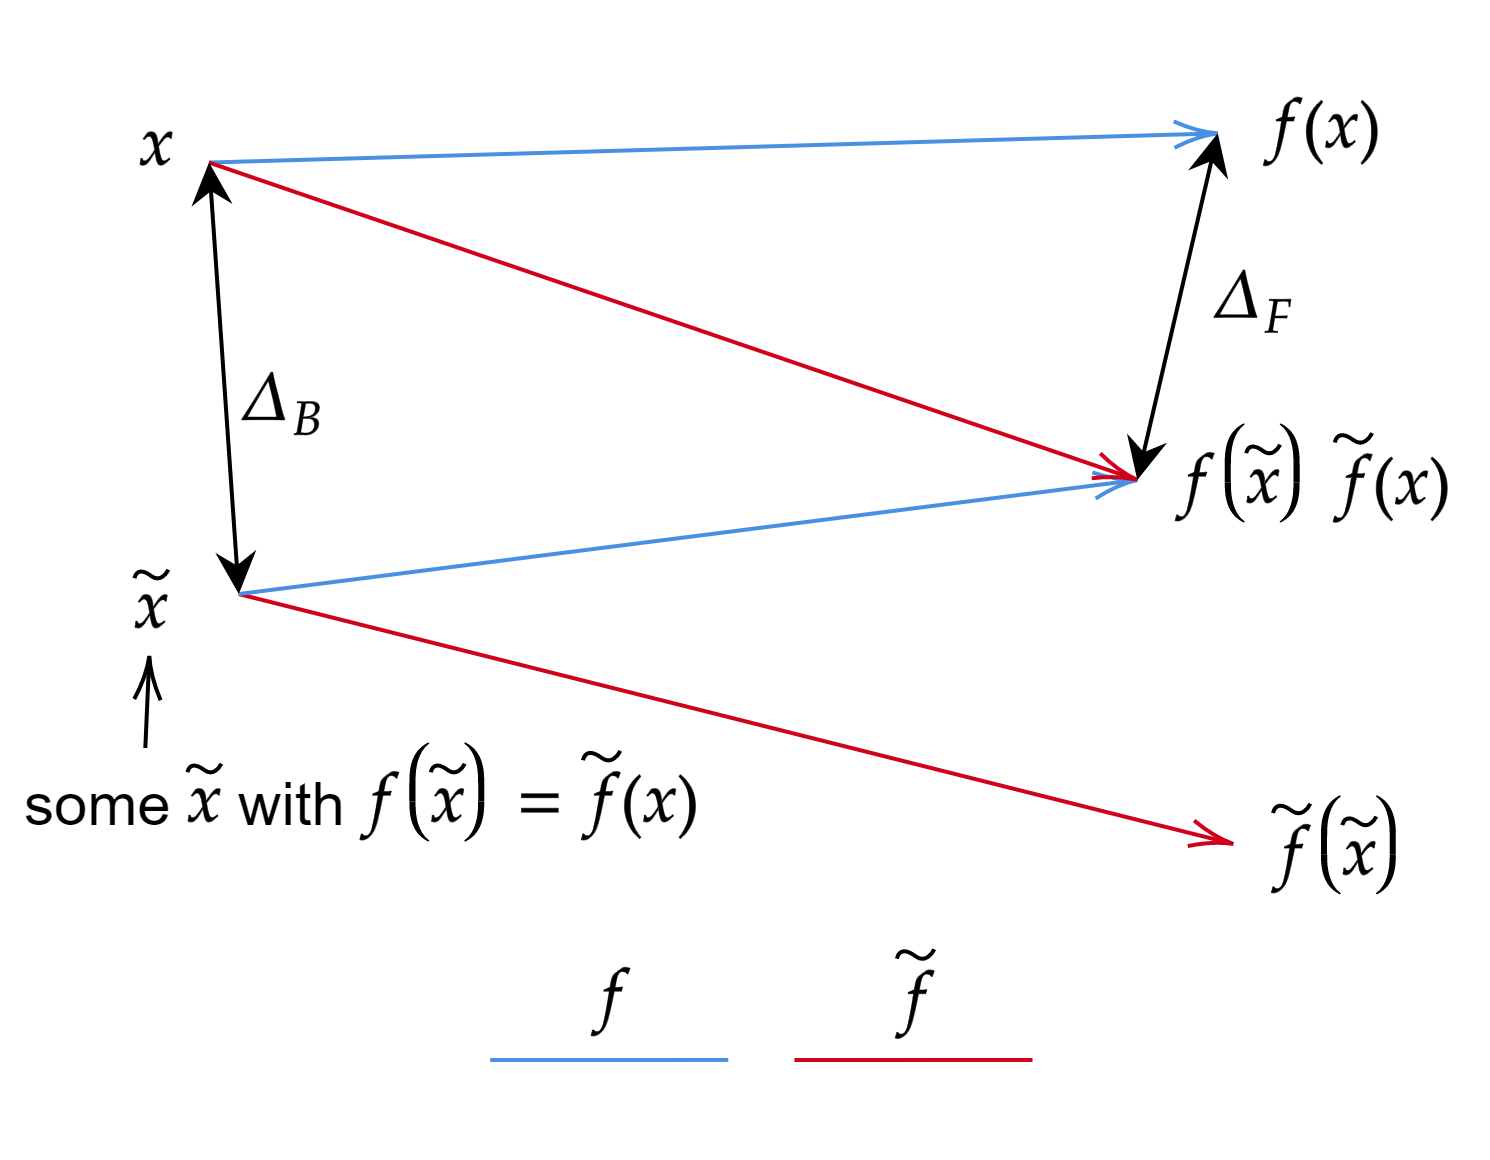
\includegraphics[width=0.45\linewidth]{sections/images/ForwardError.png}
    \caption{Illustration of Forward/Backward Error}
\end{figure}

\end{itemize}
    \item (Forward) Stability: An algorithm $ \tilde{f} $ is stable if \index{Forward Stability}
    \begin{align}
        \dfrac{\Vert \tilde{f}(x)-f(\tilde{x})\Vert }{\Vert f(\tilde{x})\Vert }=O(\varepsilon _\mathrm{machine} ),\,\forall \dfrac{\Vert \tilde{x}-x\Vert }{\Vert x\Vert }=O(\varepsilon _\mathrm{machine} ) 
    \end{align}
    \item Condition Number of problem $ f $:\index{Condition Number}
    \begin{itemize}[topsep=2pt,itemsep=0pt]
        \item Absolute condition number:
        \begin{align}
            \hat{\kappa }(x)=\lim_{\varepsilon \to 0}\mathop{\sup}\limits_{\Vert \delta x\Vert <\varepsilon }\dfrac{\Vert\delta f(x)\Vert}{\Vert\delta x\Vert}=\left\Vert \dfrac{\partial^{} f}{\partial x^{}}\right\Vert   
        \end{align}
        \item Relative condition number:
        \begin{align}
            \kappa (x)=\lim_{\varepsilon \to 0} \mathop{\sup}\limits_{\Vert \delta x\Vert <\varepsilon }\dfrac{\Vert \delta f\Vert \big/\Vert f\Vert }{\Vert \delta x\Vert \big/\Vert x\Vert }
        \end{align}
    \end{itemize}

    (Relative) Condition Number of Matrix $ \mathop{A}\limits_{m\times m}  $: 
    \begin{itemize}[topsep=2pt,itemsep=0pt]
        \item $ f(x)\equiv Ax $:
        \begin{align}
            \kappa =\Vert A\Vert \dfrac{ \Vert x\Vert }{\Vert Ax\Vert }\leq \Vert A\Vert \Vert A^{-1}\Vert  
        \end{align}
        \item $ f(b)\equiv  $ solving $ Ax=b $
        
        \begin{align}
            \kappa = \Vert A^{-1}\Vert \dfrac{\Vert b\Vert }{\Vert x\Vert }\leq \Vert A^{-1}\Vert \Vert A\Vert 
        \end{align}
    \end{itemize}
    
        Thus for matrix $ A $, denote 
        \begin{align}
            \kappa  (A)\equiv \Vert A\Vert\Vert A^{-1}\Vert 
        \end{align}
        
    \begin{itemize}[topsep=2pt,itemsep=0pt]
        \item For $ \ell_2 $ norm $ \Vert\cdot\Vert_2 $: $ \kappa (A)=\dfrac{\sigma  _1}{\sigma  _m} $\footnote{Knowledge about matrix norm see \autoref{SubSubSectionMatrixNotationAndLemma}}
    \end{itemize}
\end{itemize}


    
\subsubsection{Iteration Algorithm}
    Iteration methods are used especially for problems without analytical solution, to obtain a numerical solution.

    Iteration method: for problem $ f $ with solution $ x^* $ design an iteration function $ g $: $ X\to X $ so that 
    \begin{align}
        \lim_{n\to\infty}g^{\{n\}}(x)=\lim_{n\to\infty}\mathop{\underbrace{g(g(g(\ldots g(g}}\limits_{n}(x))\ldots ))) =x^*
    \end{align}
    
    then get solution by setting initial input value $ x^{(0)} $ and calculate $ x^{(t+1)}=g(x^{(t)}) $ repeatedly until convergence as approximate solution.
    
\begin{point}
    Three Steps for Iteration:
\end{point}

\begin{algorithm}{General Steps for Iteration}
    \begin{enumerate}[topsep=2pt,itemsep=2pt]
        \item Starting: set $ x^{(0)} $, more trials to initial value is recommended
        \item Updating: $ x^{(t+1)}=g(x^{(t)}) ,\,\forall t=0,1,2,\ldots$
        \item Stopping: when to stop, can choose various stopping criterion, e.g.
        \begin{itemize}[topsep=2pt,itemsep=0pt]
            \item Absolute convergence criterion
            \begin{align}
                |x^{(t+1)}-x^{(t)}|<\varepsilon  
            \end{align}
            
            \item Relative convergence criterion
            \begin{align}
                \dfrac{|x^{(t+1)}-x^{(t)}|}{|x^{(t)}|}< \phi 
            \end{align}
            
            \item Relative convergence criterion (2), avoid $ x^{(t)}=0 $
            \begin{align}
                \dfrac{|x^{(t+1)}-x^{(t)}|}{|x^{(t)}|+\xi }< \phi 
            \end{align}        
        \end{itemize}
    \end{enumerate}
\end{algorithm}
    



    
\begin{point}
    Convergence Order and Convergence Rate
\end{point}\index{Convergence Order}

    For each iteration value $ x^{(t)} $, define iteration error as $ \varepsilon ^{(t)}\equiv x^{(t)}-x^* $. Then an iteration method $ \lim_{t\to \infty}\varepsilon ^{(t)}=0 $ has convergence order $ \alpha  $ and convergence rate $ c $ as:
    \begin{align}
        \lim_{t\to\infty}\dfrac{|\varepsilon ^{(t+1)}|}{|\varepsilon ^{(t)}|^\alpha }=c 
    \end{align}
    
     A large $ \alpha  $ and small $ c $ declare a quick convergence.(Large $ \alpha  $ is needed more)

    Comment: Actually convergence rate and order are generally dependent on specific problem, so we usually estimate $ \alpha  $, $ c $ using some approximation/scaling to represent a generally case.

\subsubsection{Constrained Optimize Theory}
\begin{point}
    Primal Problem\index{Primal Problem}
\end{point}


    For optimize problem in convex set $ \mathcal{X} $
\begin{align}
        \mathop{\arg\min}\limits_{x\in\mathcal{X}}\quad &f(x)\tag{P}\\
        s.t.\quad   &g_i(x)\leq 0,\quad i=1,2,\ldots,k\\
        & h_j(x)=0,\quad j=1,2,\ldots,l
\end{align}

    which is called the \textbf{primal problem} for optimization.\index{Primal Problem}
    
    The \textbf{generalized Lagrange function} for primal problem defined as \index{Generalized Lagrange Function}
\begin{equation}\label{EqaGeneralizedLagrangeFunction}
 \begin{aligned}
    \mathcal{L}(x,\kappa ,\lambda )\equiv& f(x)+\sum_{i=1}^k\kappa _ig_i(x)+\sum_{j=1}^l\lambda _jh_j(x) \\
    w.r.t. \quad&\kappa _i\geq 0,\quad i=1,2,\ldots,k
\end{aligned}   
\end{equation}

        
    and we could further define a function of $ x $:
\begin{align}
    \theta _P(x)\equiv& \mathop{\max}\limits_{\kappa ,\lambda :\kappa _i\geq 0}\mathcal{L}(x,\kappa ,\lambda ) =\begin{cases}
            f(x)&\text{constraint } g,\,h \text{ satisfied}\\
            +\infty &\text{contraint unsatisfied}
        \end{cases}
\end{align}
       
    which means we can give the solution value of primal problem (P) simply by minimizing $ \theta _P(x) $, minimum denoted $ p^* $
    \begin{align}
        p^* \equiv \mathop{\min}\limits_{x}\theta _P(x)=\mathop{\min}\limits_{x}  \mathop{\max}\limits_{\kappa ,\lambda :\kappa _i\geq 0}\mathcal{L}(x,\kappa ,\lambda )
    \end{align}
    
\begin{point}
    Dual Problem\index{Dual Problem}
\end{point}

    Similar to primal problem, we can define a function of $ \kappa ,\lambda  $:
\begin{align}
    \theta _D(\kappa ,\lambda )\equiv&\mathop{\min}\limits_{x} \mathcal{L}(x,\kappa ,\lambda )
\end{align}

    and similarly get the \textbf{dual problem} of primal, value denoted $ d^* $\index{Lagrange Dual Problem}\index{Dual Problem}
\begin{align}
    d^*\equiv\max_{\kappa ,\lambda :\kappa \geq 0}\theta _D(\kappa ,\lambda )=\max_{\kappa ,\lambda :\kappa \geq 0}\mathop{\min}\limits_{x} \mathcal{L}(x,\kappa ,\lambda )
\end{align} 
    
    it is obvious that 
    \begin{align}
        d^*= \max_{\kappa ,\lambda :\kappa \geq 0}\mathop{\min}\limits_{x} \mathcal{L}(x,\kappa ,\lambda ){\color{red}\leq }\mathop{\min}\limits_{x}  \mathop{\max}\limits_{\kappa ,\lambda :\kappa _i\geq 0}\mathcal{L}(x,\kappa ,\lambda )=p^*
    \end{align}
    
\begin{point}
    Karush-Kuhn-Tucker Condition (KKT Condition)\index{KKT Condition (Karush-Kuhn-Tucker Condition)}
\end{point}

    KKT condition to allow $ d^*=p^* $ at $ (x^*,\kappa ^*,\lambda ^*) $: in the case that
\begin{itemize}[topsep=2pt,itemsep=0pt]
    \item $ f(x) $ and $ g_i(x) $ are convex
    \item $ h_j(x) $ in the form of affine function $ A_jx+b $
    \item $ g_i(x) $ are feasible constraints
\end{itemize}

    then $ \mathrm{KKT}\,\Leftrightarrow\, p^*=d^*=\mathcal{L}(x^*,\kappa ^*,\lambda ^*)  $.

    the KKT conditions are:
\begin{equation}\label{EqaKKTCondition}
    \begin{aligned}
    &\nabla_x\mathcal{L}(x^*,\kappa ^*,\lambda ^*)=0&\\
    &\kappa ^*_ig_i(x^*)=0&i=1,2,\ldots,k\\
    &g_i(x^*)\leq 0&i=1,2,\ldots,k\\
    &\kappa _i\geq 0&i=1,2,\ldots,k\\
    &\lambda _j(x^*)=0&j=1,2,\ldots,l
    \end{aligned}
\end{equation}

    
    
    
     







\subsection{Algebratic Problem in Statistics}\label{SubSectionAlgebraticProblemInStatistics}
   Considering the data structure and algorithm implement, many fundamental problems in statistics are basically algebratic problem, e.g.

\begin{itemize}[topsep=2pt,itemsep=0pt]
    \item Matrix multiplication:
    
    \begin{align}
        y=Ax,\,\text{solve } y 
    \end{align}
    \item Linear equation solution:
    \begin{align}
        b=Ax=\sum_{i=1}^nx_ia_i,\, \text{solve } x
    \end{align}
    \item OLS solution:
    \begin{align}
        \hat{\beta }=(X'X)^{-1}XY 
    \end{align}
\end{itemize}

    Generally speaking matrix $ A $ can be constructed in an arbitrary form, so an algorithm implementation needs \textbf{matrix composition} so that we have a better form to handle.
    




\subsubsection{Matrix Operation}
\begin{itemize}[topsep=2pt,itemsep=0pt]
    \item Inverse Matrix: Inverse matrix of $ A=[a_1,\ldots,a_m] $ satisfies
    \begin{align}
        A^{-1}A=AA^{-1}=I 
    \end{align}

    then $ Ax=b\Leftrightarrow x= A^{-1}b$    

    Or generally speaking, solve inverse matrix $ A^{-1}=[\alpha_1,\ldots,\alpha _m] $ is solving linear equations 
    \begin{align}
        A\alpha _i=e_i
    \end{align}
    
    In the view of column space transfrom, $ A $ and $ A^{-1} $ are mappings between space $ \mathrm{span}\{e_1,\ldots,e_m\}  $ and $ \mathrm{span}\{a_1,\ldots,a_m\}  $, i.e.
    \begin{align}
        \mathrm{span}\{e_1,\ldots,e_m\} \mathop{\rightleftharpoons }\limits_{A^{-1}b}^{Ax}  \mathrm{span}\{a_1,\ldots,a_m\}
    \end{align}
    
    \item Unitary Matrix: Furthur for unitary $ A $, denoted as $ Q $ with $ QQ^*=I $, is an orthonormal transformation.
\begin{itemize}[topsep=2pt,itemsep=0pt]
    \item $ |Q|=1 $ for rotation, $ |Q|=-1 $ for reflection.
    \item $ \lambda_Q=\pm 1 $
    \item Geometric structure preserved, e.g. inner product and norm.
\end{itemize}

    \item Projection: \index{Projection Operator}
    \begin{itemize}
        \item Basic definition of projector $ P_X $: idempotent matrix, project onto hyperplane $ X $ 
        \begin{align}
            P_X^2=P_X 
        \end{align}        
        \item Complementary projector $ I-P_X $: onto the complementary space of $ X $
        \begin{align}
             (I-P)^2=I-P
        \end{align}
        \item Orthogonal Projection: Projector such that $ Pv\perp (I-P)v $. Thm.: $ Pv\perp (I-P)v\Leftrightarrow P^*=P $
        
        Derivation: Projection of vector $ v $ on hyperplane $ X $ satisties (denoted as $ Xp $)
        \begin{align}
            0=\langle Xp,Xp-v\rangle=p^*X^*(Xp-v)\Rightarrow p=(X^*X)^{-1}Xv\Rightarrow Xp={\color{red}X(X^*X)^{-1}X}v={\color{red}P_X}v
        \end{align}
        
        More Properties of orthogonal projector see \autoref{SubSubSectionStatisticalInferenceInMultiLRA}.
        \item Orthogonal projector onto vector $ q $:
        \begin{align}
            P_q=q(q^*q)^{-1}q^*=\dfrac{qq^*}{\Vert q \Vert^2_2 } 
        \end{align}
        
        
    \end{itemize}



\end{itemize}

% \subsubsection{Solution to System of Equations}
%     Solve system of linear equations:
%     \begin{align}
%         x=\arg\{Ax=b\} 
%     \end{align}
    
% \begin{itemize}[topsep=2pt,itemsep=0pt]
%     \item $ LU $ decomposition algorithm:
%     \begin{enumerate}[topsep=2pt,itemsep=2pt]
%         \item 
%     \end{enumerate}
    
        
%     \item $ QR $ decomposition algorithm:
%     \begin{enumerate}[topsep=2pt,itemsep=2pt]
%         \item Use e.g. Householder reflector to compute a $ QR $ decomposition of $ A $:
%         \begin{align}
%             A=QR\Rightarrow QRx=b 
%         \end{align}
        
%         \item Use orthonormality of $ Q $: computation complexity $ \sim 2mn^2-\dfrac{2}{3}n^3 $
%         \begin{align}
%             Rx=Q^*b =\xi
%         \end{align}
%         \item Solve $ Rx-\xi  $ to get $ x $.
        
        
%     \end{enumerate}
    
        
% \end{itemize}

    






\subsubsection{Projection and Least Square Problem}
    Recall: Linear model $ Y=X\beta +\varepsilon  $, basically solving linear equation $ Y=X\beta  $, however generally $ Y\notin \mathrm{span}(X)  $, then we use OLS method to reach an estimation of $ \beta$    :
    \begin{align}
        \hat{\beta }=\mathop{\arg\min}\limits_{\beta }\Vert Y-X\beta  \Vert^2
    \end{align}
    
    where for $ \Vert \cdot \Vert = \ell_2 $-norm, $ X\hat{\beta } $ is the projection of $ X\beta  $ onto hyperplane $ X $:
    \begin{align}
        X\hat{\beta }= X(X^*X)^{-1}X^*Y\equiv HY=P_XY
    \end{align}

    For non-full rank $ A=X^*X $: use pseudoinverse $ A^+=(A^*A)^{-1}A^* $
    
    % Derivation: Projection of vector $ v $ on hyperplane $ X $ satisties (denoted as $ Xp $)
    % \begin{align}
    %      0=<Xp,Xp-v>=p^*X^*(Xp-v)\Rightarrow p=(X^*X)^{-1}Xv\Rightarrow Xp=X(X^*X)^{-1}Xv=P_Xv
    % \end{align}
    
    % Properties:(see \autoref{SubSubSectionStatisticalInferenceInMultiLRA})
    % \begin{itemize}[topsep=2pt,itemsep=2pt]
    %     \item Hermite: $ P_X^*=P_X $;
    %     \item Idempotence: $ P_X^2=P_X $
    %     \item Rank: $ \mathrm{rk}(P_X)=tr(P_X)=\mathrm{rk}(X)$
    %     \item Space of $ P $:
    %     \begin{itemize}[topsep=2pt,itemsep=0pt]
    %         \item $ \mathrm{Im}(I-P)=\mathcal{N}(P) $
    %         \item $ \mathrm{Im}(P)=\mathcal{N}(I-P)  $
    %     \end{itemize}
    % \end{itemize}
    
    % Projection on vector $ q $:
    % \begin{align}
    %     P_q=q(q^*q)^{-1}q^*=\dfrac{qq^*}{\Vert q \Vert } 
    % \end{align}


\begin{point}
    Task of OLS (Linear Model): Solve $ \hat{\beta }=(X^*X)^{-1}X^*Y $, or equivalently solve $ X^*X\hat{\beta }=X^*Y $
\end{point}

    Note: size of matrix denoted $ X=\mathop{X}\limits_{m\times n}  $
    % Algorithm using $ QR $ decomposition:
\begin{itemize}[topsep=2pt,itemsep=0pt]
    \item Cholesky decomposition algorithm: computation complexity $ \sim mn^2+\dfrac{n^3}{3} $
    \begin{enumerate}[topsep=2pt,itemsep=2pt]
        \item Use Cholesky decomposition for $ X^*X $:
        \begin{align}
            A^*A=R^*R\Rightarrow R^*R\hat{\beta }=X^*Y 
        \end{align}
        \item Solve $ \xi =\arg\{ R^*\xi =X^*Y \} $:
        \begin{align}
            R^*R\hat{\beta }=X^*Y=R^*\xi \Rightarrow R\hat{\beta }=\xi  
        \end{align}
        \item Solve $ R\hat{\beta }=\xi  $ to get $ \hat{\beta } $
    \end{enumerate}
    \item $ QR $ decomposition algorithm: computation complexity $ \sim 2mn^2-\dfrac{2}{3}n^3 $
    \begin{enumerate}[topsep=2pt,itemsep=2pt]
        \item Use e.g. Householder Reflection algorithm to compute $ X=QR $
        \item use the orthonormal property of $ Q $:
        \begin{align}
            X^*X\hat{\beta }=X^*Y\Rightarrow R^*Q^*QR\hat{\beta }=R^*R\hat{\beta }=R^*Q^*Y\Rightarrow R\hat{\beta }=Q^*Y 
        \end{align}
        \item Solve $ R\hat{\beta }=Q^*Y $ to get $ \hat{\beta } $
    \end{enumerate}
    \item SVD algorithm: computation complexity $ \sim 2mn^2+11n^3 $
    \begin{enumerate}[topsep=2pt,itemsep=2pt]
        \item Compute SVD of $ X $: $ X=U\Sigma V^* $
        \begin{align}
             X^*X\hat{\beta }=X^*Y\Rightarrow V\Sigma ^2V^*\hat{\beta }=V\Sigma U^*Y\Rightarrow \Sigma V^*\hat{\beta }=U^*Y
        \end{align}
        \item Solve $ \hat{\beta }=V\Sigma ^{-1}U^*Y $ to get $ \hat{\beta } $
    \end{enumerate}
    
\end{itemize}
    
    Algorithm comparison \& trade-off: faster $ \leftrightsquigarrow $ less stable.



\subsubsection{Gaussian $ LU $ Decomposition \& Cholesky Decomposition}
\begin{point}
    Gaussian Elimination Algorithm
\end{point}

    Gaussian Elimination decomposes matrix $ A $ as lower triangular matrix $ \times $ upper triangular matrix
    \begin{align}
        \mathop{A}\limits_{m\times m}=\mathop{L}\limits_{m\times m}\mathop{U}\limits_{m\times m}  =
        \begin{bmatrix}
            *&&&\\
            *&*&&\\
            \vdots&\vdots&\ddots&\\
            *&*&\ldots&*
        \end{bmatrix}
        \begin{bmatrix}
            *&*&\ldots &*\\
            &*&\ldots&*\\
            &&\ddots&\vdots\\
            &&&*
        \end{bmatrix}  
    \end{align}
    
    Conducted by continuously row transformation of $ A $:
    \begin{align}
        L_{m-1}\ldots L_2L_1A=L^{-1}A=U 
    \end{align}
    
    where each $ L_i $ corresponds to a gauss elimination operation such that $ \left[L_i(L_{i-1}\ldots L_2L_1A)\right]_{i+1:m,i}=0 $, with $\left[L_i(L_{i-1}\ldots L_2L_1A)\right]_{1:i,:} $ fixed. $ L_i $ has the form as 
    \begin{align}
        L_i=I-l_ie_i^*,\qquad l_i=[0,\ldots,l_{i+1,i},\ldots,l_{m,i}]^T\quad l_{j,i}=A_{ji}/A_{ii}
    \end{align}
    
    Then we have $ L=L_1^{-1}L_2^{-1}\ldots L_{m-1}^{-1}U $, with $ U=L_{m-1}\ldots L_2L_1A $

    If some pivot element $ (L_{i-1}\ldots L_1A)_{ii}=0 $, use a row transformation $ P_i $ such that $ (P_iL_{i-1}\ldots L_1A)_{ii}\neq 0 $, thus $ LU $ decomposition is expanded as 
    \begin{align}
        L_{m-1}P_{m-1}\ldots L_2P_2L_1P_1A=U
    \end{align}

    Good properties of $ L_i=I-l_ie_i^* $: enable a quick algorithm implement of $ LU $ decomposition:
    \begin{itemize}[topsep=2pt,itemsep=0pt]
        \item Inverse of $ L_i $:
        \begin{align}
            L_i^{-1}=(I-l_ie_i^*)^{-1}=I+l_ie_i^* 
        \end{align}
        \item Multiplication of $ L_i^{-1} $:
        \begin{align}
            L_i ^{-1}L_{i+1}^{-1}=(I+l_ie_i^*)(I+l_{i+1}e_{i+1}^*)=I+l_ie_i^*+l_{i+1}e_{i+1}^*
        \end{align}
        \item Interchangeability of $ P_i $ and $ L_j $ :
        % (note that $ P_i^2=I $):
        \begin{align}
            L_{m-1}P_{m-1}\ldots L_2P_2L_1P_1=(\tilde{L}_{m-1}\ldots\tilde{L}_2\tilde{L}_1)(P_{m-1}\ldots P_2P_1),\qquad \tilde{L}_i=P_{m-1}\ldots P_{i+1}L_iP^{-1}_{i+1}\ldots P^{-1}_{m-1}
        \end{align}        
        where note that $ P_{k} $ only exchange row/column $ k $ and $ \kappa>k $, thus $ \tilde{L}_i $ is still left triangular.
    \end{itemize}
    
    \noindent Thus get expression of $ LU $ decomposition $ PA=LU $:
    \begin{align}
         PA=LU\quad\begin{cases}
            P=P_{m-1}\ldots P_2P_1\\
            L= (\tilde{L}_{m-1}\ldots\tilde{L}_2\tilde{L}_1)^{-1}\\
            \tilde{L}_i=P_{m-1}\ldots P_{i+1}L_iP_{i+1}\ldots P_{m-1}\\
            U=L_{m-1}P_m\ldots L_2P_2L_1P_1A
         \end{cases} 
    \end{align}
    
    

    Complexity of Gaussian Elimination:
    \begin{align}
        \mathrm{flops}_\mathrm{GE}=&\sum_{i=1}^{m-1}\sum_{k=i+1}^m 2(m-i+1)\sim \dfrac{2}{3}m^3
    \end{align}
 
\begin{point}
    Cholesky Decomposition
\end{point}

    Hermitian positive-definite matrix $ A $ can $ LU $ decompose as
    \begin{align}
        A=LU=R^*R
    \end{align}
    
    Algorithm: write $ A $ in partitioned matrix then conduct symmetric row/column transformation
    
\begin{align}
    A=&\begin{bmatrix}
      1&w_1^*\\
      w_1&K
    \end{bmatrix}
    \\
    =&\begin{bmatrix}
    1&0\\w_1&I
    \end{bmatrix}
    \begin{bmatrix}
    1&0\\0&K-w_1w_1^*
    \end{bmatrix}
    \begin{bmatrix}
    1&w_1^*\\0&I
    \end{bmatrix}\\
    =&R_1^*K_1R_1
  \end{align} 
    

    Note that $ K_1 $ is still hermite positive-definite, we can repeat the above process
    
        \begin{align}
            K_1=&\
            \begin{bmatrix}
            1&0\\0&K-w_1w_1^*
            \end{bmatrix}\\
            =&\begin{bmatrix}
            1&0&0\\
            0&1&0\\
            0&w_2&I
            \end{bmatrix}
            \begin{bmatrix}
            1&0&0\\
            0&1&0\\
            0&0&K-w_1w_1^*-w_2w_2^*
            \end{bmatrix}
            \begin{bmatrix}
            1&0&0\\
            0&1&w_2^*\\
            0&0&I
            \end{bmatrix}\\
            =&R_2^*K_2R_2
          \end{align} 
    

    repeat untill $ K_m=I $: $ A=(R_mR_{m-1}\ldots R_1)^*I(R_mR_{m-1}\ldots R_1)=R^*R $
    
    Complexity of Cholesky Decomposition:
    \begin{align}
        \mathrm{flops}_\mathrm{CD}=&\sum_{i=1}^{m}\sum_{k=i}^m 2(m-k+1)+1 \sim \dfrac{1}{3}m^3
    \end{align}
 
    
    









    



\subsubsection{$ QR $ Decomposition: Gram-Schmidt/Householder/Givens Method}
    
    $ QR $ Decomposition: Orthogonal Triangularization of matrix $ A $
\begin{align}
    \mathop{A}\limits_{m\times n} =\mathop{Q}\limits_{m\times n} \mathop{R}\limits_{n\times n}     
\end{align}


\begin{align}
    A=\begin{bmatrix}
        a_1&\ldots &a_n
    \end{bmatrix} 
    =QR=
    \begin{bmatrix}
        q_1&\ldots&q_n
    \end{bmatrix}
    \begin{bmatrix}
        r_{11}&r_{12}&\ldots&r_{1n}\\
        &r_{22}&\ldots&r_{2n}\\
        &&\ddots&\vdots\\
        &&&r_{nn}
    \end{bmatrix}
\end{align}

    Every $ \mathop{A}\limits_{m\times n} \in \mathbb{C}^{m\times n} $ ($ m\geq n $) has $ QR $ decomposition, specially:
    \begin{itemize}[topsep=2pt,itemsep=0pt]
        \item Full decomposition exists
        \item Reduced decomposition with $ r_{ii}>0 $ is unique.
        % \item If $ A\in\mathbb{R}^{m\times n} $, then $ U\in\mathbb{R}^{m\times n} $, 
    \end{itemize}
    
        
% \Leftrightarrow\begin{cases}
    %     Q=AR^{-1}&\mathrm{span}\text{ of }A\\
    %     R=Q^{-1}A&\text{Orthogonal Triangularization}
    % \end{cases} 
    Here introduce 3 kinds of algorithm:
    \begin{itemize}[topsep=2pt,itemsep=0pt]
        \item \hyperlink{GS-Decomposition}{Gram-Schmidt Orthogonalization}: $ \sim O(2mn^2) $, sequentially orthogonalizes the columns of $ A $, traditional way
        \item[$ \color{red}\star $] \hyperlink{Householder-Reflection}{Householder Reflection}: $ \sim O(2mn^2-\dfrac{2}{3}n^3) $, most commonly used, stable for ill \& dense matrix
        \item \hyperlink{Givens-Rotation}{Givens Rotation}: $ \sim O(3mn^2-n^3) $, used for sparse matrix, e.g. Hessenberg matrix
    \end{itemize}
    
        




\begin{point}
    \hypertarget{GS-Decomposition}{(Classical) Gram-Schmidt Orthogonalization}\index{CGS (Classical Gram-Schmidt Orthogonalization)}
\end{point}

    Key idea: project $ a_i $ onto $ \mathrm{span}\{q_1,\ldots,q_{i-1}\}^\perp  $ as $ q_i $, with $ q_1 $ initialized as $ \hat{a}_1 $, projection coefficient $ r_{ij} $ forms $ R $.

    For each projection, the projector matrix is 
    \begin{equation}\label{EqaCGSProjector}
        P_i=I-\sum_{k=1}^{i-1}q_kq_k^*      
    \end{equation}
    
    expression of $ q_i $ and $ r_{ij} $: 

\begin{align}
    r_{ij}=\begin{cases}
        q_i^*a_j&i\neq j\\
        \Vert a_i-\sum_{k=1}^{i-1}r_{ki}q_k \Vert& i=j 
    \end{cases}\qquad 
    q_i=\dfrac{a_i-\sum_{k=1}^{i-1}r_{ki}q_k}{r_{ii}}=\dfrac{a_i-\sum_{k=1}^{i-1}q_kq_k^*a_i}{\Vert a_i-\sum_{k=1}^{i-1}q_kq_k^*a_i \Vert }
\end{align}

    Note: Algorithm implementation of $ q_i $ is $ (q_{<i})\to r_{k<i,i}\to q_{i}\& r_{ii} \to (q_{>i}) $


\begin{point}
    Modified Gram-Schmidt Orthogonalization Algorithm\index{MGS (Modified Gram-Schmidt Orthogonalization)}
\end{point}

    In \autoref{EqaCGSProjector}, projection of G-S orthogonalization for each $ a_i $ is conducted `simultaneously', while modified G-S decomposition is conducted step by step.

\begin{align}
    P_i=I-\sum_{k=1}^{i-1}q_kq_k^*=\prod_{k=1}^{i-1}(I-q_kq_k^*) 
\end{align}
    
    Decomsition result are the same, but modified algorithm is more stable for numerical computation, avoid problem of recursive $ q_i $.


\begin{rcode}
    Algorithm of CGS/MGS
\begin{lstlisting}[language=R]
GS <- function(A,MGS=FALSE){
    stopifnot(is.matrix(A))
    m <- dim(A)[[1]]
    n <- dim(A)[[2]]
    v=matrix(0,nrow = m,ncol=m)
    r=matrix(0,nrow = m,ncol=n)
    q=matrix(0,nrow = m,ncol=m)
    for(j in 1:n){
        v[,j] <- A[,j]
        if(j>1){
        for(i in 1:(j-1)){
          r[i,j]=sum(q[,i]*ifelse(MGS,v[,j],A[,j]))#对MGS取v,CGS取a
          v[,j] <- v[,j]-r[i,j]*q[,i]
        }}
        r[j,j] <- sqrt(sum(v[,j]^2))
        q[,j] <- v[,j]/r[j,j]
    }
  return(list(q,r))
}
\end{lstlisting}
\end{rcode}






\begin{point}
    \hypertarget{Householder-Reflection}{Householder Reflection}
\end{point}

    Key idea: Reflect $ A_{i:m,i} $ onto $ e_{1}\in\mathbb{C}^{m-i+1} $ as a vector of the same length $ \Vert  A_{i:m,i} \Vert e_{1}\in\mathbb{C}^{m-i+1} $ (later we denote the $ l^\mathrm{th}  $ unit vector $ e_{l}\in\mathbb{C}^{m-i+1}\equiv e_{m-i+1,l} $), reflector $ F_i $ in $ \mathbb{C}^{(m-i+1)\times (m-i+1)} $ and auxiliary vector $ v_i $:\footnote{Here $ \mathrm{sgn}() $ for reflecting toward $ -e_1 $/$ e_1 $.}
    \begin{align}
        \mathbb{C}^{(m-i+1)\times( m-i+1)} \ni F_i=I_{m-i+1}-2\dfrac{vv^*\,}{\Vert v \Vert_2^2 }\qquad v= \mathrm{sgn}(A_{i,i}) \Vert  A_{i:m,i} \Vert e_{m-i+1,1}+ A_{i:m,i} 
    \end{align}

    where $ \mathrm{sgn}(\cdot) $ corresponds to reflection onto $ \hat{e} $ or $ -\hat{e} $.   
    Reflector on $ A\in\mathbb{C}^{m\times n} $:
    \begin{align}
        Q_i=\begin{bmatrix}
            I_{i-1}&0\\
            0&F_i
        \end{bmatrix} 
    \end{align}
    
    and $ QR $ calculated by (note that $ F^2=I_{m-i+1} $)
    \begin{align}
        R=Q_n\ldots Q_2Q_1A\qquad Q=Q_1Q_2\ldots Q_n
    \end{align}
    
    

    Householder Reflection is more stable than Gram-Schimidt Orthogonalization


    
    
    Error of Householder Reflection $ A=\tilde{Q}\tilde{R}+E $, residual is controlled by $ \Vert E \Vert \leq \Vert A \Vert O(\varepsilon _\mathrm{machine}) $

    Mainly caused by stability and accuracy of orthogonal matrix $ \tilde{Q} $.
    % GS: $ a $


\begin{rcode}
\lstinline|R.| uses Householder Reflection to conduct $ QR $ decomposition.
\begin{lstlisting}[language=R]
A.qr <- qr(A)
Q <- qr.Q(A.qr)
R <- qr.R(A.qr)
\end{lstlisting}
\end{rcode}

\begin{point}
    \hypertarget{Givens-Rotation}{Givens Rotation}
\end{point}
    
    Key idea: use rotation
    \begin{align}
        Rx=\begin{bmatrix}
            \cos\theta &-\sin\theta \\
            \sin\theta &\cos\theta 
        \end{bmatrix} \begin{bmatrix}
            x_i\\x_j
        \end{bmatrix}=\begin{bmatrix}
            \sqrt{x_i^2+x_j^2}\\0
        \end{bmatrix}
        \Leftrightarrow \begin{cases}
            \cos\theta =\dfrac{x_i}{\sqrt{x_i^2+x_j^2}}\\
            \sin\theta =\dfrac{x_j}{\sqrt{x_i^2+x_j^2}}
        \end{cases}
    \end{align}
    
    act on $ A_{i-1:i,j:n} $ so that $ A_{i,j}=0 $, each time use two rows to create 1 zero. Slow, used for special sparse matrix.
    
\subsubsection{Eigenvalue Decomposition}
    For square matrix $ A \in\mathbb{C}^{m\times m}$, its eigenvector is the vector $ x_i $ whose direction (subspace) is invariant under transform operator $ A $.
    \begin{align}
        Ax_i =\lambda _ix_i
    \end{align}
    
    Properties:
\begin{itemize}[topsep=2pt,itemsep=0pt]
    \item Determinant and trace of $ A $:
    \begin{align}
        \det(A)=\prod_{i=1}^m\lambda _i\qquad tr(A)=\sum_{i=1}^m\lambda _i 
    \end{align}
    \item $ x_i $ for special kinds of $ A $: if $ \mathrm{span}\{q_i\}=\mathbb{C}^m  $, then (generally $ X $ is \textbf{not} orthogonal)
    \begin{align}
        AX=X\Lambda \Rightarrow  A=X\Lambda X^{-1} 
    \end{align}
    
    
    Further for $ AA^*=A^*A $ (Normal Matrix\index{Normal Matrix} 规范矩阵. Include: hermitian $ A=A^* $\index{Hermitian Matrix}, skew hermitian $A=-A^* $, unitary $ A^{-1}=A^* $, circulant matrix\index{Circulant Matrix}\footnote{Circulant Matrix, or similarly Latin Square.
    \begin{align}
        C=\begin{bmatrix}
            c_0&c_1&c_2&c_3\\
            c_3&c_0&c_1&c_2\\
            c_2&c_3&c_0&c_1\\
            c_1&c_2&c_3&c_0
        \end{bmatrix} 
    \end{align}
    
    }, and such $ A+kI $), orthonormality of $ x_i\to q_i $:
    \begin{align}
        \langle q_i,q_j  \rangle =\delta_{ij}
    \end{align}
    Eigenvalue Decomposition/Spectrum Decomposition, $ X\to Q $:
    \begin{align}
        AQ=Q\Lambda \Rightarrow A=Q\Lambda Q^{-1}=Q\Lambda Q^*
    \end{align}
    \item Eigenvalue decomposition and positive definite matrix (Gershgorin circle thm.), $ \lambda _i $ falls in neighbourhood of $ a_{ii} $:
    \begin{align}
        D(\lambda_i,a_{ii})<\sum_{j=1,j\neq i}^m|a_{ij}| 
    \end{align}
    \item Rayleigh quotient:
    \begin{align}
        \max R(A,q)\equiv \max \dfrac{q^*Aq}{q^*q}=\lambda _1 
    \end{align}
    
    
        
\end{itemize}

    






Eigenvactor Algorithm: Power method to find leading eigen pair.

for independent eigenvectors $ x_i $ and an arbitrary vector $ \xi =\sum_{i=1}^mc_ix_i $:
\begin{align}
    A^k\xi =A^k\sum_{i=1}^mc_ix_i=\sum_{i=1}^mc_i\lambda_i^kx_i=c_1\lambda _1^k\left[x_1+\sum_{i=2}^n\dfrac{c_i}{c_1}\left(\dfrac{\lambda _i}{\lambda _1}\right)^kx_i\right]\to c_1\lambda _1^kx_1
\end{align}




\begin{algorithm}{Basic Eigen Decomposition}
    \begin{enumerate}[topsep=2pt,itemsep=0pt]
    \item pick a random $ q_0 $
    \item compute normalized $ \dfrac{Aq_i}{\Vert Aq_i \Vert }=q_{i+1} $
    \item repeat until $ \Vert q_{i-1}-q_{i-2} \Vert<\varepsilon_\mathrm{preset}    $
    \item $ q_i $ as the eigenvector, $ q_i^TAq_i\approx q_i^T\lambda_1 q_i=\lambda _1 $
\end{enumerate}
\end{algorithm}
    


    This algorithm requires $ |\lambda _1|>|\lambda _2|\geq\ldots  $ for quick convergence.
    













\subsubsection{SVD Decomposition}
\begin{point}
    SVD (Singular Value Decomposition)\index{SVD (Singular Value Decomposition)} Form:
\end{point}

    
\begin{itemize}[topsep=2pt,itemsep=0pt]
    \item Reduced Form:
\begin{align}
    \mathop{A}\limits_{m\times n} =\mathop{U}\limits_{m\times n}\mathop{\Sigma }\limits_{n\times n}\mathop{V^*}\limits_{n\times n}     
\end{align}

\begin{align}
    A=\begin{bmatrix}
        a_1&\ldots &a_n
    \end{bmatrix} 
    =U\Sigma V^*=
    \begin{bmatrix}
        u_1&\ldots&u_n
    \end{bmatrix}
    \begin{bmatrix}
        \sigma_1&&&\\
        &\sigma_2&&\\
        &&\ddots&\\
        &&&\sigma_n
    \end{bmatrix}
    \begin{bmatrix}
        v_1^*\\
        v_2^*\\
        \vdots\\
        v_n^*
    \end{bmatrix}
\end{align}
    \item Full Form:

    \begin{align}
        \mathop{A}\limits_{m\times n} =\mathop{U}\limits_{m\times m}\mathop{\Sigma }\limits_{m\times n}\mathop{V^*}\limits_{n\times n}     
    \end{align}
    
    \begin{align}
        A=\begin{bmatrix}
            a_1&\ldots &a_n
        \end{bmatrix} 
        =U\Sigma V^*=
        \begin{bmatrix}
            u_1&u_2&\ldots&u_m
        \end{bmatrix}
        \begin{bmatrix}
            \sigma_1&&&\\
            &\sigma_2&&\\
            &&\ddots&\\
            &&&\sigma_n\\
            0&0&0&0\\
            \vdots&\vdots&\vdots&\vdots
        \end{bmatrix}
        \begin{bmatrix}
            v_1^*\\
            v_2^*\\
            \vdots\\
            v_n^*
        \end{bmatrix}
    \end{align}
\end{itemize}


    Existence and uniqueness of SVD:
\begin{itemize}[topsep=2pt,itemsep=0pt]
    \item Every $ A\in\mathbb{C}^{m\times n} $ has SVD with $ \{\sigma_i\} $ unique
    \begin{align}
        A=U\Sigma V^* =\sum_{i=1}^n\sigma _iu_iv_i^*
    \end{align}
    
    \item if $ A $ is squared, then $ U,V $ determined
    \item if $ A\in\mathbb{R}^{m\times n} $, then $ U,V \in \mathbb{R}$ 
\end{itemize}

\begin{point}
    SVD Expression
\end{point}

    $ U $, $ V $ are eigenvectors of $ AA^* $, $ A^*A $ respectively
\begin{align}
    A^*A=V\Sigma ^2V^*\qquad AA^*=U\Sigma ^2U^*\qquad u_j=\dfrac{Av_j}{\sigma _j}\quad \sigma _j=\sqrt{\lambda _{A^*A}}=\sqrt{\lambda _{AA^*}}
\end{align}

\begin{point}
    Properties of SVD:
\end{point}

   
\begin{itemize}[topsep=2pt,itemsep=0pt]
    \item rank of $ A $: $ r=\mathrm{rk}(\mathop{A}\limits_{m\times n} )=\# \text{ non-zero } \sigma _i  $
    \item Space of $ A  $:
    \begin{itemize}
        \item $ \mathcal{R}(A)=\mathrm{span}\{u_1,\ldots ,u_r\}  $
        \item $ \mathcal{C}(A)=\mathrm{span}\{v_1,\ldots,v_r\}  $
        \item $ \mathcal{N}(A)=\mathrm{span}\{v_{r+1},\ldots,v_n\}  $
    \end{itemize}
    \item Norm:
    \begin{itemize}[topsep=2pt,itemsep=0pt]
        \item Euclidean Norm: $ \Vert A \Vert _2=\sigma _1 $
        \item Frobenius Norm: $ \Vert A \Vert _F=\sqrt{\sum_{i=1}^r\sigma _i^2 } $
        \item Nuclear Norm: $ \Vert A \Vert _*=\sum_{i=1}^r\sigma _i $
    \end{itemize}
    \item Square matrix:
    \begin{itemize}
        \item if $ A=A^* $, then $ \sigma _j=|\lambda _A|_j $
        \item $ \det(A)=\prod_{i=1}^m\sigma _i $
    \end{itemize}
    \item Low-rank Approximation of $ A $ using SVD:
    \begin{align}
        A_k= \sum_{i=1}^k\sigma _iu_iv_i^*=A-\sum_{j=k+1}^r\sigma _ju_jv_j^*
    \end{align}
    
    is the `nearest' rank $ k $ matrix from $ A $ 
    \begin{align}
        \mathop{\min}\limits_{\mathrm{rk}(\Xi)=k }\Vert A-\Xi \Vert _2=\Vert A-A_k \Vert _2=\sigma _{k+1}  
    \end{align}
    
\end{itemize}

\begin{point}
    When $ A $ is positive definite, SVD and ED get the same result.
\end{point}

\begin{align}
    A=Q\Lambda Q^*\Rightarrow  A=Q\mathrm{sgn}(\Lambda )|\Lambda |Q^*=U\Sigma Q^*=U\Sigma V^* 
\end{align}



\subsubsection{Schur Decomposition}
    Unitary Triangularization of matrix $ A $ (always exists in $ \mathbb{C}^{m\times m} $):
    \begin{align}
        A=QTQ^*,\, Q\text{ unitary, }T\text{ upper-triangular} 
    \end{align}
    
    for $ A\in\mathbb{R}^{m\times m} $: $ T $ is quasi-triangular, diag of $ T $ is $ \mathrm{Re} (\lambda _i) $
















\subsection{Numeric Optimization Algorithm I}

Algorithm Optimization in Statistics: e.g.
\begin{itemize}[topsep=2pt,itemsep=0pt]
    \item MLE Maximazation
    \item Linear/Logistics Regression: Minimizing error
    \item Clustering: minimizing within-cluster distance \& maximizing between-cluster distance
    \item Box-Cox $ \lambda  $ determining
    \item Machine Learning Model training, minimizing loss function
\end{itemize}

\begin{point}
Duality of Optimization and Rooting:
\end{point}

\begin{itemize}[topsep=2pt,itemsep=0pt]
    \item Optimization: e.g. minimizing function $ g(x) $:
    \begin{align}
        \arg\min g(x) \leftrightharpoons \arg\{\nabla g(x)=0\}
    \end{align}
    \item Rooting: extract root $ f(x)=0 $:
    \begin{align}
        \arg \{f(x)=0\}\leftrightharpoons \arg\min f(x)^Tf(x) 
    \end{align}   
\end{itemize}

    More specific example: expand function to $ 2^\mathrm{nd}  $ as $ g(x)\approx\dfrac{1}{2}x^TAx-bx+c $ (differnetiation of quadric $ x^TAx $ see \autoref{SubSubSectionMatrixNotationAndLemma})
    \begin{align}
        \arg\min\dfrac{1}{2}x^TAx-bx+c\leftrightharpoons \arg\{\dfrac{A+A^T}{2}x=b\}
    \end{align}


    \fbox{
        \begin{minipage}{0.9\linewidth}
            $ \Delta $ i.e. for optmizing task $ \arg\min g(x) $, we can either minimizing $ g(x) $, or rooting $ f(x)\equiv \nabla g(x) $
        \end{minipage}
    }\\
    
    
\begin{point}
    Algorithm Design Aim:
\end{point}

\begin{itemize}[topsep=2pt,itemsep=0pt]
    \item Robustness: can be applied on various problems
    \item Accuracy: reach solution with great precision, at the same time insensitive to machine error
    \item Efficiency: computer time/storage not required
\end{itemize}

\begin{point}
    Iteration in Optimization Problem
\end{point}

    Usually iteration is used in optmizing problem, by approximate solution $ x^* $ step by step. 
\begin{itemize}[topsep=2pt,itemsep=0pt]
    \item Bracketing method means the solution $ x^* $ is always within some iteration interval $ I^{(t)}=[x_\mathrm{left},x^*,x_\mathrm{right}  ] $, use convergence condition $ m(I^{(t)})<\varepsilon  $ to obtain solution.
    
    % Includes: Golden Search/Fibonacci Serach/Bisection Search/Regula Falsi
    \item Open method: Not necessarily $ x^*\in I^{(t)} $, but convergence using $ d(x^{(t)},x^{(t-1)})<\varepsilon  $. Usually faster than bracketing, but less stable, and sensitive to initial value.
    
    % Includes: Newton Raphson/Secant
    \item Hybird Method: Mixture of bracketing and open according to iteration step feature
    
    % Includes: Brent's method
\end{itemize}







\begin{point}
    Content
\end{point}
\begin{itemize}[topsep=2pt,itemsep=0pt]
    \item \hyperlink{GoldenSection}{Golden Section \& Fibonacci Section Search}: Bracketing method direct search for minimizer;
    \item \hyperlink{Bisection}{Bisection Search}: Bracketing method direct search for root
    \item \hyperlink{Interpolation}{Interpolation Method}: Include either bracketing/open method, approximate function to obtain root/minimizer
    \begin{itemize}[topsep=2pt,itemsep=0pt]
        \item \hyperlink{RegulaFalsi}{Regula Falsi}: Bracketing linear interpolation for rooting
        \item \hyperlink{Secant}{Secant Interpolation}: Open linear interpolation for rooting
        \item \hyperlink{ParabolicInterpolation}{Parabolic Interpolation}: Open parabolic interpolation for minimizing
        \item \hyperlink{InverseQuadric}{Inverse Parabolic Interpolation (IQI)}: Open interpoation for rooting
    \end{itemize}
    
    \item \hyperlink{HybridMethod}{Hybrid Method}: Combination of bracketing method and open interpolation method for rooting. Include Dekker's and Brent's, most used method
    \begin{itemize}[topsep=2pt,itemsep=0pt]
        \item \hyperlink{Dekker}{Dekker's Method}: Hybrid of bisection and secant interpolation method for rooting
        \item[$\color{red}\star$] \hyperlink{Brent}{Brent's Method}: Hybrid of bisection, secant interpolation and IQI for rooting
    \end{itemize}
       
    \item \hyperlink{FixedPoint}{Fixed Point Iteration Method}: Open method for rooting, including univariate and multivariate linear case.
    \begin{itemize}[topsep=2pt,itemsep=0pt]
        \item Univariate Fixed Point Iteration
        \item \hyperlink{JacobiMethod}{Jacobi Method}
        \item \hyperlink{GaussSeidelMethod}{Gauss Seidel Method}
        \item \hyperlink{SORMethod}{Successive Over-Relaxation Method}
    \end{itemize}
    
        
    \item[$\color{red}\star$] \hyperlink{Simplex}{Nelder-Mead Method/Simplex Method}: Open method for minimizer based on simplex iteration
\end{itemize}

    
\begin{point}
    Default Methods in \lstinline|R.| 
\end{point}
\begin{itemize}[topsep=2pt,itemsep=0pt]
    \item \lstinline|optim(VEC_OF_INI_VAR,FUN)|: Nelder-Mead Simplex search method, use \lstinline|method=c('Nelder-Mead',|\\\lstinline|'BFGS','L-BFGS-B','CG','SANN','Brent')| to choose different methods
    \item \lstinline|uniroot(FUN,INTERVAL)|: Brent's Method;
    \item \lstinline|optimize(FUN,INTERVAL)|: Golden Section+Parabolic Interpolation.
\end{itemize}

    
    % \lstinline|optim()|函数默认方法为Nelder-Mead单纯形搜索法。\lstinline|uniroot()|默认用Brent's方法 \lstinline|optimize()|函数默认方法为Golden Section+二次插值法





\subsubsection{Golden Section/Fibonacci Section Search}
\index{Golden Section Search}\index{Fibonacci Section Search}
    \hypertarget{GoldenSection}{Problem}: minimizing univariate function $ g(x) $, within a pre-estimated interval $ [x_1^{(0)},x_4^{(0)}] $. For $ f $ that is undiffernetiable/complicated to compute, this method is often used. 

    Basic idea: within a unimodal interval $ I^{(0)}=[x_1^{(0)},x_4^{(0)}] $ of $ f(x) $, pick two symmetric points $ x_2^{(0)},x_3^{(0)} $ in $ I_0 $ so that 
\begin{equation}\label{EqaRExpressionInGolden}
    x_2^{(0)}-x_1^{(1)}=x_4^{(0)}-x_3^{(0)}=(1- r^{(0)})(x_4^{(0)}-x_1^{(0)}) \quad  r^{(t)}>1/2
\end{equation}
    
    then extreme point should falls in one of $ [x^{(t)}_1,x^{(t)}_3] $ or $ [x^{(t)}_2,x^{(t)}_4] $, iteration the interval by comparing $ g(x_2) $ and $ g(x_3) $: use one of them as the next interval. And for less computation, we hope that one of $ g(x_2^{(t)}) $ of $ g(x_3^{(t)}) $ can be used in step $ t+1 $ as $ g(x_3^{(t+1)}) $ or $ g(x_2^{(t+1)}) $, i.e.
    \begin{align}
        \text{if }g(x_2^{(t)})>g(x_3^{(t)}):&\, [x_1^{(t+1)},x_2^{(t+1)},x_4^{(t+1)}]:= [x_2^{(t)},x_3^{(t)},x_4^{(t)}]\\
        \text{if }g(x_2^{(t)})\leq g(x_3^{(t)}):&\, [x_1^{(t+1)},x_3^{(t+1)},x_3^{(t+1)}]:= [x_1^{(t)},x_2^{(t)},x_3^{(t)}]
        \end{align}


        also use \autoref{EqaRExpressionInGolden}, we have (here use $g(x_2^{(t)})> g(x_3^{(t)}) $ case for derivation)
        \begin{align}
            r^{(t+1)}=\frac{x_4^{(t)}-x_2^{(t)}}{x_4^{(t)}-x_1^{(t)}}=\dfrac{x_4^{(t+1)}-x_2^{(t+1)}}{x_4^{(t+1)}-x_1^{(t+1)}}=\dfrac{x_4^{(t)}-x_3^{(t)}}{x_4^{(t)}-x_2^{(t)}}=\dfrac{1-r^{(t)}}{r^{(t)}}
        \end{align}
        

\begin{algorithm}{Golden Section/Fibonacci Section Search}

\begin{enumerate}[topsep=2pt,itemsep=2pt]
    \item Initialize $ I^{(0)}=[x_1^{(0)},x_4^{(0)}] $ with $ x^*\in I^{0} $
    \item For each step $ x^{(t)} $:
    \begin{enumerate}[topsep=2pt,itemsep=2pt]
        \item Calculate $ r^{(t)} $, and then $ g(x_2^{(t)}) $, $ g(x_{3}^{(t)}) $
        \item compare $ g(x_2^{(t)}) $ and $ g(x_3^{(t)}) $, and update interval    
        \begin{align}
            \text{if }g(x_2^{(t)})>g(x_3^{(t)}):&\, [x_1^{(t+1)},x_2^{(t+1)},x_4^{(t+1)}]\equiv [x_2^{(t)},x_3^{(t)},x_4^{(t)}]\\
            \text{if }g(x_2^{(t)})\leq g(x_3^{(t)}):&\, [x_1^{(t+1)},x_3^{(t+1)},x_4^{(t+1)}]\equiv [x_1^{(t)},x_2^{(t)},x_3^{(t)}]
        \end{align}
    \end{enumerate}
    \item Repeat until convergence $ m(I^{(t)})<\varepsilon  $
\end{enumerate}
    
    % For less computation, we hope that one of $ g(x_2^{(t)}) $ of $ g(x_3^{(t)}) $ can be used in step $ t+1 $ as $ g(x_3^{(t+1)}) $ or $ g(x_2^{(t+1)}) $, i.e.

    Choice of $ r^{(t)} $: for algorithm robustness and avoid ill sequence, we will usually use some special $ r^{(t)} $:
\begin{itemize}[topsep=2pt,itemsep=0pt]
    \item Golden Section Search: use $ r^{(t)}=r=\mathrm{const}$, such $ r $ should satisfies
    \begin{align}
        r=\dfrac{1-r}{r}\Rightarrow r=\dfrac{\sqrt{5}-1}{2}=\dfrac{1}{\phi }\approx 0.618
    \end{align}

    Convergence at  
    \begin{align}
         m(I^{(t)})=r^{t}m(I^{(0)})<\varepsilon
    \end{align}
    
    
    
    \item Fibonacci Section Search: choose for $ t=0 $ as $ r^{(0)}=\dfrac{F_{n-1}}{F_{n}} $, where $ \{F_n\} $ is Fibonacci sequence, then
\begin{align}
    r^{(0)}=&\dfrac{F_{n-1}}{F_n}\\
    r^{(1)}=&\dfrac{1-r^{(0)}}{r^{(0)}}=\dfrac{F_{n-2}}{F_{n-1}}\\
    r^{(2)}=&\dfrac{1-r^{(1)}}{r^{(1)}}=\dfrac{F_{n-3}}{F_{n-2}}\\
    \vdots&\\
    r^{(t)}=&\dfrac{F_{n-t-1}}{F_{n-t}}\\
    \vdots&\\
    r^{(n-3)}=&\dfrac{F_2}{F_3}=\dfrac{1}{2}\,\text{(the last step of iteration)}
\end{align}
    
    To determine the preset $ n $, first use convergence condition 
    \begin{align}
         m(I^{(n-2)})=\prod_{i=0}^{n-3}r^{(i)}m(I^{(0)})=\dfrac{F_2}{F_n}m(I^{(0)})<\varepsilon \Rightarrow \begin{cases}
             F_n>\dfrac{m(I^{(0)})}{\varepsilon }\\
             F_{n-1}<\dfrac{m(I^{(0)})}{\varepsilon }
         \end{cases}
    \end{align}
    
    then conduct iteration, using $ r^{(t)}=\dfrac{F_{n-t-1}}{F_{n-t}} $.
    
\end{itemize}

    
\end{algorithm}
    


    Basically the two methods have similar background, noticing that the eigen equation of Fibonacci sequence is $ x^2=x+1 $, and $ \lim_{n\to \infty}\dfrac{F_{n-1}}{F_n}=\dfrac{\sqrt{5}-1}{2}=\dfrac{1}{\phi } $\footnote{General Formula of Fibonacci sequence:
    \begin{align}
        F_n=\dfrac{1}{\sqrt{5}}\left( (\phi )^n-(-\dfrac{1}{\phi })^n \right) 
    \end{align}
    }

    Can be proven: Golden section need one more iteration call than Fibonacci section:
    \begin{align}
        n_\mathrm{GS}=n_\mathrm{Fib}+1 
    \end{align}

    Convergence order $ \alpha =1 $, rate $ c=\dfrac{1}{\phi } $


 
\subsubsection{Bisection Search Method}
    % Gradient methods are suitable for derivable function $ f $, minimizing $ f $ is equivalent to root finding of $ \nabla f $
\index{Bisection Search}
    \hypertarget{Bisection}{Problem}: rooting univariate function $ f(x) $, with a pre-­estimated interval $ I^{(0)}=[x_1^{(0)},x_2^{(0)}] $, with $ f(x_1^{(0)})f(x_2^{(0)})<0 $

    Idea: Intermediate value thm.: for continuous $ f:[a,b]\to \mathbb{R}  $, $ f(a)f(b)<0\Rightarrow \exists x^*, s.t. f(x^*)=0 $. 

\begin{algorithm}{Bisection Search}
    
\begin{enumerate}[topsep=2pt,itemsep=2pt]
    \item Initialize $ I^{(0)}=[x_1^{(0)},x_2^{(0)}] $ satisfying $ f(x_1^{(0)})f(x_2^{(0)})<0 $
    \item In each iteration $ x^{(t)} $:
    \begin{enumerate}[topsep=2pt,itemsep=2pt]
        \item compute midpoint function value
    \begin{align}
        x_m^{(t)}=\dfrac{1}{2}\left(x_1^{(t)}+x_2^{(t)}\right) 
    \end{align}
        \item update interval according sign of $ f(x_m^{(t)}) $:
    \begin{align}
        I^{(t+1)}=[x_1^{(t+1)},x_2^{(t+1)}]:=\begin{cases}
            [x_1^{(t)},x_m^{(t)}],& f(x_1^{(t)})f(x_m^{(t)})<0\\
            [x_m^{(t)},x_2^{(t)}],& f(x_m^{(t)})f(x_2^{(t)})<0
        \end{cases} 
    \end{align}
    \end{enumerate}

    \item Repeat until convergence $ m(I^{(t)})<\varepsilon  $
\end{enumerate}
\end{algorithm}
    



    Convergence order $ \alpha =1 $, rate $ c=\dfrac{1}{2} $.


\subsubsection{Interpolation Methods: Linear/Quadratic/Lagrange Interpolation}
\index{Interpolation}
    \hypertarget{Interpolation}{Interpolation} is an approximation to function, thus can get approximation to solution. Interpolation can be used for both minimizing or root finding.

\begin{point}
    \hypertarget{RegulaFalsi}{Regula Falsi/Linear Interpolation (Bracketing) for Root Finding}: 
\end{point}
    
    Idea of regula falsi linear interpolation: at root $ x^* $ of $ f(x) $:
    \begin{align}
        f(x) \approx\left. \dfrac{\mathrm{d}^{} f}{\mathrm{d}x^{}}\right|_{x^*}(x-x^*)
    \end{align}
    
    Iterate by repeatedly constructing linear interpolation/secant and use the root as an approximation to $ x^* $.

\begin{algorithm}{Regula Falsi Interpolation}
    \begin{enumerate}[topsep=2pt,itemsep=2pt]
        \item Initialize interval $ I^{(0)}=[x_1^{(0)},x_2^{(0)}] $ with $ f(x_1^{(0)})f(x_2^{(0)})<0 $
        \item In each iteration $ x^{(t)} $:
        \begin{enumerate}[topsep=2pt,itemsep=2pt]
            \item Compute linear interpolation of $ (x_1^{(t)},f(x_1^{(t)})),(x_2^{(t)},f(x_2^{(t)})) $, and compute the root of the straight line
            \begin{align}
                x_r^{(t)}=\dfrac{x_1^{(t)}f(x_2^{(t)})-x_2^{(t)}f(x_1^{(t)})}{f(x_2^{(t)})-f(x_1^{(t)})}
            \end{align}
        
            compute $ f(x_r^{(t)}) $
            \item update interval according to sign of $ f(x_r^{(t)}) $:
            \begin{align}
                I^{(t+1)}=[x_1^{(t+1)},x_2^{(t+1)}]:=\begin{cases}
                    [x_1^{(t)},x_r^{(t)}],& f(x_1^{(t)})f(x_r^{(t)})<0\\
                    [x_r^{(t)},x_2^{(t)}],& f(x_r^{(t)})f(x_2^{(t)})<0
                \end{cases} 
            \end{align}
        \end{enumerate}
        \item Repeat until convergence $ m(I^{(t)})<\varepsilon  $
    \end{enumerate}
\end{algorithm}
    



    Note: for enough steps of iteration $ t_\xi  $, the iteration would be short enough such that $ \mathrm{sgn}(f''(x))=\mathrm{const} $, in which case one of $ x_1^{(t)} $ or $ x_2^{(t)} $ would remain fixed for $ t>t_\xi  $.\footnote{For $ f''(x)f'(x)>0 $, $ x_2 $ fixed; $ f''(x)f'(x)<0 $, $ x_1 $ fixed.}

    Convergence order $ \alpha =1 $, rate $ c=-\dfrac{f''(x^*)}{2f'(x^*)}(x^*-x_\mathrm{fixed} ) $. Note that sign dependency of $ x_\mathrm{fixed}  $  on $ f''(x) $ and $ f'(x) $ ensures $ c>0 $.

\begin{point}
    \hypertarget{Secant}{Secant Interpolation/Linear Interpolation (Open)} for Root Finding
\end{point}    

    Instead of limiting $ x^*\in[x_1^{(t)},x_2^{(t)}] $ (bracketing) by ensuring $ f(x_1^{(t)})f(x_2^{(t)})<0 $, we can also remove the restrict, i.e. just use the latest two points to construct secant.

\begin{algorithm}{Secant Interpolation}

\begin{enumerate}[topsep=2pt,itemsep=2pt]
    \item Initialize two points  $ x^{(-1)},\,x^{(0)} $.(interval not necessarily include potential root $ \hat{x}^* $)
    \item In each iteration $ x^{(t)} $:
    \begin{enumerate}[topsep=2pt,itemsep=2pt]
        \item Compute linear interpolation of $ (x^{(t-1)},f(x^{(t-1)})),\,(x^{(t)},f(x^{(t)})) $
        \item Use the root to update $ x^{(t+1)} $:
    \begin{align}
        x^{(t+1)}=\dfrac{x^{(t-1)}f(x^{(t)})-x^{(t)}f(x^{(t-1)})}{f(x^{(t)})-f(x^{(t-1)})}
    \end{align}
    \end{enumerate}
    
    \item Repeat until convergence, .e.g. $ |x^{(t)}-x^{(t-1)}|<\varepsilon  $
\end{enumerate}

   
\end{algorithm}
    

    Comment: For interval small enough such that $ \mathrm{sgn}(f''(x))=\mathrm{const} $ and $ f(x^{(t)})f(x^{(t-1)})<0 $, this method might goes back to bracketing linear interpolation.

    Convergence order $ \alpha \approx 1.618 $.

\begin{point}
    \hypertarget{ParabolicInterpolation}{Parabolic Interpolation for Minimizing}
\end{point}

    Idea of parabolic interpolation: at extreme point $ x^* $, function $ f $ has taylor series
    \begin{align}
        g(x)\approx g(x^*)+\dfrac{1}{2}\left.\dfrac{\mathrm{d}^{2} g}{\mathrm{d}x^{2}}\right|_{x^*}(x-x^*)^2
    \end{align}
    
    we can iteration by repeatedly construct parabola to approximate $ f(x^*)+\dfrac{1}{2}\left.\dfrac{\mathrm{d}^{2} f}{\mathrm{d}x^{2}}\right|_{x^*}(x-x^*)^2 $ and use the exterme point of the parabola.

\begin{algorithm}{Parabolic Interpolation}

\begin{enumerate}[topsep=2pt,itemsep=2pt]
    \item First initialize three point $ (x_1^{(0)},x_2^{(0)},x_3^{(0)}) $,
    \item In each iteration $ x^{(t)} $:
    \begin{enumerate}[topsep=2pt,itemsep=2pt]
        \item Use $ (x_1^{(t)},x_2^{(t)},x_3^{(t)}) $ to compute corresponding $ f(x) $, then use quadric fitting to obtain parabola $ \Gamma^{(t)} $
    \item Replace $ \max\{x_1^{(t)},x_2^{(t)},x_3^{(t)}\} $ by extreme point of $ \Gamma ^{(t)} $ to update as $  (x_1^{(t+1)},x_2^{(t+1)},x_3^{(t+1)}) $
    \end{enumerate}
    \item Repeat until convergence.
\end{enumerate}
    
\end{algorithm}
    
    Convergence order $ \alpha \approx 1.3247 $.
    

% \begin{rcode}
% \begin{lstlisting}[language=R]
% optimize(FUN,lower = ,upper = )
% \end{lstlisting}
% \end{rcode}

\begin{point}
    Lagrange Polynomial Interpolation\index{Lagrange Polynomial Interpolation}
\end{point}

    Lagrange Polynomial is a function base set: Given $ n+1 $ point $ (x_0,y_0),\ldots,(x_n,y_n) $ ($ n\geq 1 $), Lagrange polynomial:
\begin{align}
    \ell_i=\prod_{j=1,j\neq i}^n\dfrac{x-x_j}{x_i-x_j},\quad i=0,1,\ldots,n
\end{align}

    And Lagrange interpolation function: $ L(x)=\sum_{i=0}^ny_i\ell_i $

    $ n=1 $ for linear interpolation, $ n=2 $ for parabolic interpolation.


\begin{point}
    \hypertarget{InverseQuadric}{Inverse Parabolic Interpolation (IQI)}:\index{IQI (Inverse Parabolic Interpolation)} Open interpoation for rooting
\end{point}

    Note that general parabola $ y=\dfrac{1}{2}ax^2+bx+c $ might have 0 or 2 root simultaneously, thus use inverse quadric function $ x=\dfrac{1}{2}ay^2+by+c $, i.e. inverse quadric interpolation.

\begin{algorithm}{Inverse Parabolic Interpolation}
    \begin{enumerate}[topsep=2pt,itemsep=2pt]
        \item First initialize three point $ C^{(0)}=\left(x^{(-2)},x^{(-1)},x^{(0)}\right) $
        \item In each iteration $ x^{(t)} $:
        \begin{enumerate}[topsep=2pt,itemsep=2pt]
            \item Use $ C^{(t)}=\left(x^{(t-2)},x_2^{(t-1)},x_3^{(t)}\right) $ to compute IQI function, and get root 
        \begin{align}
            s=\sum_{\mathrm{cycle}\,x^{(t-2)},x^{(t-1)},x^{(t)}}\dfrac{x^{(t-2)}f(x^{(t-1)})f(x^{(t)})}{\left[f(x^{(t-2)})-f(x^{(t-1)})\right]\left[f(x^{(t-2)})-f(x^{(t)})\right]}
        \end{align}
        \item Update points
        \begin{align}
             C^{(t+1)}=\left(x^{(t-1)},x^{(t)},x^{(t+1)}\right)=\left( x^{(t-1)},x^{(t)},s \right)
        \end{align}
        \end{enumerate}
        \item Repeat until convergence $ |x^{(t)}-x^{(t-1)}|<\varepsilon  $
    \end{enumerate}
\end{algorithm}
    


    


\subsubsection{Hybrid Method: Dekker's/Brent's}
\hypertarget{HybridMethod}{}

\begin{point}
    \hypertarget{Dekker}{Dekker's Method}\index{Dekker's Method}
\end{point}

    Dekker's method is a hybrid of open linear interpolation and bisection, in each step, use one of interpolation/bisection according to iteration condition to achieve both quick convergence and stability.
\begin{algorithm}{Dekker's Method}

\begin{enumerate}[topsep=2pt,itemsep=2pt]
    \item Initialize three point $ a^{(0)},\,b^{(0)},\, b^{(-1)}=a^{(0)} $, where interval bteween $a^{(0)},\,b^{(0)} $ should include potential root $ \hat{x}^{*} $, i.e. $ f(a^{(0)})f(b^{(0)})<0 $
    \item In each iteration $ x^{(t)} $:
    \begin{enumerate}[topsep=2pt,itemsep=2pt]
        \item $ a^{(t)},\,b^{(t)} $ is labelled as follows: label ensure $ |f(a^{(t)})|\geq |f(b^{(t)})| $, thus $ b^{(t)} $ is the estimate of root, while $ a^{(t)} $ is the `contrapoint' of $ b^{(t)} $
        \item compute root $ s $ of linear interpolation of $ (a^{(t)},f(a^{(t)})), \, (b^{(t)},f(b^{(t)})) $, and compare with midpoint $ m=\dfrac{a^{(t)}+b^{(t)}}{2} $
        % , say $ X^{(t+1)}:(x^{(t+1)},f^{(t+1)}) $, where 
        \begin{align}
            \tilde{b}^{(t+1)}= 
            \begin{cases}
                s=\dfrac{a^{(t)}f(b^{(t)})-b^{(t)}f(a^{(t)})}{f(b^{(t)})-f(a^{(t)})},&s\in [m,b^{(t)}]\,(\text{or }[b^{(t)},m])\\
                m=\dfrac{a^{(t)}+b^{(t)}}{2},&s\notin [m,b^{(t)}]\,(\text{or }[b^{(t)},m])
            \end{cases}
        \end{align}
        \item Then update $ \tilde{a}^{(t+1)} $ as one of $ a^{(t)} $ and $ b^{(t)} $, such that $ f(\tilde{a}^{(t+1)})f(\tilde{b}^{(t)})<0 $, then relabel $ \tilde{a}^{(t+1)} $, $ \tilde{b}^{(t)} $ to $ a^{(t+1)} $, $ b^{(t+1)} $ according to $ |f(a^{(t+1)})|>|f(b^{(t+1)})| $
    \end{enumerate}
    \item Repeat until convergence $ |b^{(t)}-b^{(t-1)}|<\varepsilon  $
\end{enumerate}

    
\end{algorithm}
    

    Comment: In step 3, the choice between bisection and open interpolation take advantage of quick convergence of open method, also ensure stability by using bisection for ill secant root $ s $. However for interval small enough, this method might also goes back to bracketing linear interpolation, then $ b^{(t)} $ convergence very slow.
    

\begin{point}
    \hypertarget{Brent}{Brent's Method}\index{Brent-Dekker Method}
\end{point}

    Brent's Method is an improvement of Dekker's Method: 
\begin{itemize}[topsep=2pt,itemsep=0pt]
    \item Avoid convergence problem of $ b^{(t)} $ in the case of bracketing linear interpolation by checking $ |b^{(t)}-b^{(t-1)}|>\delta  $ before linear interpolation, otherwise use bisection
    \item Further adding IQI interpolation if $ a^{(t)},\,b^{(t)},\,b^{(t-1)} $ are distinct for quicker convergence, root for IQI:
    \begin{align}
        s'=\sum_{\mathrm{cycle}\,a^{(t)},b^{(t)},b^{(t-1)}}\dfrac{a^{(t)}f(b^{(t)})f(b^{(t-1)})}{\left[f(a^{(t)})-f(b^{(t)})\right]\left[f(a^{(t)})-f(b^{(t-1)})\right]}
    \end{align}

\end{itemize}

\begin{rcode}
\begin{lstlisting}[language=R]
uniroot()
\end{lstlisting}
\end{rcode}




\subsubsection{Fixed Point Iteration: Univariate}
\hypertarget{FixedPoint}{}
\index{Fixed Point Iteration}
    Idea: Contraction mapping thm.: for function $ f:X\to X $ satisfying
    \begin{align}
        d(f(x),f(y))\leq \beta d(x,y),\, \beta <1 
    \end{align}
    
    then such $ f $ has a unique fixed point $ x^* $ such that $ f(x^*)=x^* $, and convergence is ensured:
    \begin{align}
        d(f^{\{n\}}(x),x^*)\leq \dfrac{\beta ^n}{1-\beta }d(f(x),x^*) 
    \end{align}
    

    For univariate function, requires $ |f'(x)|<1 $(at least at $ x $ near $ x^* $)

    To minimize $ f(x) $, i.e. find root of $ f'(x)=g(x) $, i.e. find fixed point of $ G(x)\equiv \alpha f'(x)+x=x $, requires $ |G'(x)|=|\alpha f''(x)+1|<1 $.

    Note: We can also use inverse function of $ \alpha f'(x)+x $, and further use $ G_1(x)=rG(x)+(1-r)x $ to find fixed point.

    Iteration: use $ \hat{x}^*=x^{(n)}= G^{\{n\}}(x)=\mathop{\underbrace{G(G(G(\ldots G(G}}\limits_{n}(x))\ldots ))) $, until $ |x^{(n)}-x^{(n-1)}|<\varepsilon  $

    Basically, fixed point iteration is the same as parallel chord method: use the root of $ y-g(x^{(t)})=-\dfrac{1}{\alpha } (x-x^{(t)}) $ as $ x^{(t+1)} $.

    Convergence order is $ \alpha  $ in $ G(x)=\alpha f'(x)_x $


\subsubsection{Fixed Point Iteration: Multivariate Linear}
    For solution of $ Ax=b $ using fixed point iteration, where $ AA^*=A^*A $(normal matrix), requires:
    \begin{align}
        \rho (A)=\max|\lambda |<1 
    \end{align}
    
\begin{itemize}[topsep=2pt,itemsep=0pt]
    \item \hypertarget{JacobiMethod}{Jacobi Method}: Decompose $ A=D+E $, where $ D $ is diagonal part
    \begin{align}
        \mathop{A}\limits_{n\times n} =
        \begin{bmatrix}
        a_{11}&a_{12}&\ldots&a_{1n}\\
        a_{21}&a_{22}&\ldots&a_{2n}\\
        \vdots&\vdots&\ddots&\vdots\\
        a_{n1}&a_{n2}&\ldots&a_{nn}
        \end{bmatrix}=D+E=
        \begin{bmatrix}
        a_{11}&0&\ldots &0\\
        0&a_{22}&\ldots &0\\
        \vdots&\vdots&\ddots&\vdots\\
        0&0&\ldots&a_{nn}
        \end{bmatrix}+
        \begin{bmatrix}
        0&a_{12}&\ldots&a_{1n}\\
        a_{21}&0&\ldots&a_{2n}\\
        \vdots&\vdots&\ddots&\vdots\\
        a_{n1}&a_{n2}&\ldots&0
        \end{bmatrix}
    \end{align}
    
    Then fixed point iteration: using $ (D+E)x=b \Rightarrow x^{(t+1)}=D^{-1}(b-Ex^{(t)})$
    \begin{align}
        x_i^{(t+1)}=\dfrac{1}{a_{ii}}\left(b_i-\sum_{j\neq i}a_{ij}x_j^{(t)}\right)
    \end{align}
    
    \item \hypertarget{GaussSeidelMethod}{Gauss-Seidel Method}: Decompose $ A=L+U $
    \begin{align}
        \mathop{A}\limits_{n\times n} =L+U=
        \begin{bmatrix}
        a_{11}&0&\ldots &0\\
        a_{21}&a_{22}&\ldots &0\\
        \vdots&\vdots&\ddots&\vdots\\
        a_{n1}&a_{n2}&\ldots&a_{nn}
        \end{bmatrix}
        +\begin{bmatrix}
        0&a_{12}&\ldots&a_{1n}\\
        0&0&\ldots&a_{2n}\\
        \vdots&\vdots&\ddots&\vdots\\
        0&0&\ldots&0
        \end{bmatrix}
    \end{align}

    Then fixed point iteration: using $ (L+U)x=b \Rightarrow Lx^{(t+1)}=(b-Ux^{(t)})$, iteration:
    \begin{align}
        x_i^{(t+1)}=\dfrac{1}{a_{ii}}\left(b_i-\sum_{j=1}^{i-1}a_{ij}x_j^{(t+1)}-\sum_{j=i+1}^na_{ij}x_j^{(t)}\right)
    \end{align}


    \item \hypertarget{SORMethod}{Successive Over-Relaxation Method (SOR Method)}:\index{SOR Method (Successive Over-Relaxation Method)} Decompose $ A=D+L+U $
    \begin{align}
        \mathop{A}\limits_{n\times n} =D+L+U=
        \begin{bmatrix}
        a_{11}&0&\ldots &0\\
        0&a_{22}&\ldots &0\\
        \vdots&\vdots&\ddots&\vdots\\
        0&0&\ldots&a_{nn}
        \end{bmatrix}+
        \begin{bmatrix}
        0&0&\ldots&0\\
        a_{21}&0&\ldots&0\\
        \vdots&\vdots&\ddots&\vdots\\
        a_{n1}&a_{n2}&\ldots&0
        \end{bmatrix}
        +\begin{bmatrix}
        0&a_{12}&\ldots&a_{1n}\\
        0&0&\ldots&a_{2n}\\
        \vdots&\vdots&\ddots&\vdots\\
        0&0&\ldots&0
        \end{bmatrix}
    \end{align}
        
    Then fixed point iteration: using $ \omega (D+L+U)x=\omega b \Rightarrow (D+\omega L)x=\omega b-\left[\omega U+(\omega -1)D\right])x$, move non-diagonal elements to $  \mathrm{R.H.S.} $ 
    \begin{align}
        x_i^{(t+1)}=(1-\omega )x_i^{(t)}+\dfrac{\omega }{a_{ii}}\left(b_i-\sum_{j=1}^{i-1}a_{ij}x_j^{(t+1)}-\sum_{j=i+1}^na_{ij}x_j^{(t)}\right),\qquad \omega \in(0,2)
    \end{align}

        Comment: SOR iteration step is the $ \omega  $ weighted average of $ x^{(t)} $ and Gauss-Seidel iteration.


\end{itemize}



    



\subsubsection{Nelder-Mead Method}
\index{N-M Search Method (Nelder-Mead Search Method)}\index{Simplex Search Method}\hypertarget{Simplex}{}
    For multivariate function $ g(x) $, with $ x\in \mathbb{R}^n $, usually use Nelder-Mead Method, or Simplex Search Method. Simplex is a generalization of triangle/tetrahedron to any arbitrary dimension, and Nelder-Mead method is conducted by iterating simplex.



\begin{algorithm}{Nelder-Mead Method}

\begin{enumerate}[topsep=2pt,itemsep=2pt]
    \item First initialize simplex $ C^{(0)} $ by preset $ p_0 $ and $ \vec{\lambda } $:
    \begin{align}
        C^{(0)}=\{x_0^{(0)},x_1^{(0)},\ldots ,x_n^{(0)}\}, x_0^{(0)}=p_0,\,x_i^{(0)}=p_0+\lambda _i\hat{e}_i
    \end{align}
    \item In each iteration $ x^{(t)} $:
    \begin{enumerate}[topsep=2pt,itemsep=2pt]
        \item First sort $ \{x_i^{(t)}\} $ according to $ g(x_i^{(t)}) $ as
    \begin{align}
        g(x_{(0)}^{(t)})\leq g(x_{(1)}^{(t)})\leq\ldots\leq g(x_{(n)}^{(t)})
    \end{align}
    \item Compute centroid of  $ \complement_{C^{(t)}}^{x_{(n)}^{(t)}}=\{x_{(0)}^{(t)},x_{(1)}^{(t)},\ldots,x^{(t)}_{\color{red}(n-1)}\} $
    \begin{align}
        x_g^{(t)}= \dfrac{1}{n}\sum_{i=0}^{n-1}x_{(i)}^{(t)}
    \end{align}
    
    And compute the reflection point of $ x_{(n)}^{(t)} $:
    \begin{align}
        x_r^{(t)}:=x_g^{(t)}+(x_g^{(t)}-x_{(n)}^{(t)})
    \end{align}
    
    \item Compute $ g_{(0)}^{(t)}=g(x_{(0)}^{(t)}) $, $g_{(n-1)}^{(t)}= g(x_{(n-1)}^{(t)}) $, $ g_{(n)}^{(t)}=g(x_{(n)}^{(t)}) $, $ g_{r}^{(t)}=g(x_{r}^{(t)}) $ and compare:
    \begin{itemize}[topsep=2pt,itemsep=0pt]
        \item $ g_{r}^{(t)}<g_{(0)}^{(t)} $: reflection point $ x_r^{(t)} $ is a good trial for minimizing, further try a farther point
        \begin{align}
            x_{2r}^{(t)}:= x_g^{(t)}+2(x_g^{(t)}-x_{(n)}^{(t)})
        \end{align}
    
        then iteration according to $ g_{2r}^{(t)} $:
    \begin{align}
    C^{(t+1)}=\{x_0^{(t+1)},x_1^{(t+1)},\ldots ,x_n^{(t+1)}\}\equiv\begin{cases}
         \{x_{(0)}^{(t)},x_{(1)}^{(t)},\ldots,x_{(n-1)}^{(t)},x_{2r}^{(t)}\},& g_{2r}^{(t)}<g_{r}^{(t)}\\
         \{x_{(0)}^{(t)},x_{(1)}^{(t)},\ldots,x_{(n-1)}^{(t)},x_{r}^{(t)}\},& g_{2r}^{(t)}\geq g_{r}^{(t)}
    \end{cases}
    \end{align}
        \item $ g_{(0)}^{(t)}\leq g_{r}<g_{(n-1)}^{(t)} $: better simplex but not necessarily the best, just use
    \begin{align}
    C^{(t+1)}=\{x_0^{(t+1)},x_1^{(t+1)},\ldots ,x_n^{(t+1)}\}\equiv \{x_{(0)}^{(t)},x_{(1)}^{(t)},\ldots,x_{(n-1)}^{(t)},x_{r}^{(t)}\}
    \end{align}
        
        \item $ g_{(n-1)}^{(t)}\leq g_{r}^{(t)}$: $ x_r^{(t)} $ might not optmize the simplex, conduct shrinkage:
        \begin{align}
            x_s^{(t)}:= \begin{cases}
            x_g^{(t)}+0.5(x_g^{(t)}-x_{(n)}^{(t)}),&g_{(n-1)}^{(t)}\leq g_{r}^{(t)}<g_{(n)}^{(t)}\\
            x_g^{(t)}-0.5(x_g^{(t)}-x_{(n)}^{(t)}),&g_{(n)}^{(t)}\leq g_{r}^{(t)}
            \end{cases}
        \end{align}
        
        if $ g_s^{(t)}\leq g_{(n)}^{(t)} $, suggesting a successful shrinkage, use $ g_s^{(t)} $ for iteration
        \begin{align}
            C^{(t+1)}=\{x_0^{(t+1)},x_1^{(t+1)},\ldots ,x_n^{(t+1)}\}\equiv \{x_{(0)}^{(t)},x_{(1)}^{(t)},\ldots,x_{(n-1)}^{(t)},x_{s}^{(t)}\},\, g_s^{(t)}\leq g_{(n)}^{(t)}
        \end{align}
        
         otherwise we have to update the whole simplex:
         \begin{align}
             x_0^{(t+1)}=x_0^{(t)},\, x_i^{(t+1)}=x_0^{(t)}+\dfrac{1}{2}(x_{i}^{(t)}-x_0^{(t)})
         \end{align}
    \end{itemize}
    \end{enumerate}
\end{enumerate}
    
\end{algorithm}
    
%     多元函数求极值:依次迭代各变量,每次对一个方向求极值。
% \begin{align}
%     x_1^{(t+1)}=&\mathop{\arg\min}\limits_{x_1} g(x_1,x_2^{(t)},x_3^{(t)},\ldots,x_m^{(t)})\\
%     x_2^{(t+1)}=&\mathop{\arg\min}\limits_{x_2} g(x_1^{(t+1)},x_2,x_3^{(t)},\ldots,x_m^{(t)})\\
%     \vdots&\\
%     x_m^{(t+1)}=&\mathop{\arg\min}\limits_{x_m} g(x_1^{(t+1)},x_2^{(t+1)},x_3^{(t+1)},\ldots,x_m) 
% \end{align}















\subsection{Numeric Optimization Algorithm II}
    To minimize some arbitrary function $ f(x) $, the idea of gradient iteration method is to update $ x^{(t)} $ based on (minus) gradient $ -\nabla f(x) $, with some modification on direction $ p^{(t)}=T\left(-\nabla f(x)\right) $ and step length $ \alpha ^{(t)} $
    \begin{align}
        x^{(t+1)}=x^{(t)}+\alpha ^{(t)}T\left(-\nabla f(x^{(t)})\right)=x^{(t)}+\alpha ^{(t)}p^{(t)}
    \end{align}
    
\begin{itemize}[topsep=2pt,itemsep=0pt]
    \item Modifying Direction $ p^{(t)} $:
    \begin{itemize}[topsep=2pt,itemsep=0pt]
        \item \hyperlink{GradientDescent}{Gradient Descent}: $ p^{(t)}=-\nabla f\left(x^{(t)}\right) $
        % \item 
        \item \hyperlink{NRMethod}{Newton-Raphson Method}: use Hessian matrix $ p^{(t)}=-\left[H(x^{(t)})\right]^{-1}\nabla f\left(x^{(t)}\right) $
        \item \hyperlink{FSNRMethod}{Fisher Scoring Method}: for statistics problem, use fisher information $ I\left(x^{(t)}\right)=-E_Y\left(H(x^{(t)})\right) $, $ p^{(t)}=I\left(x^{(t)}\right)^{-1}\nabla f\left(x^{(t)}\right)  $
        \item \hyperlink{QuasiNewtonMethod}{Quasi-Newton Method}: usually use secant condition to approximate Hessian $ \hat{H}^{(t)}=M^{(t)} $ or $ \hat{H^{-1}}^{(t)}=B^{(t)} $, with various updating SR-1/DFP/BFGS/L-BFGS/Broyden Class
        \item \hyperlink{SteepestDescent}{Steepest Descent}: general form based on various norm choice.
        \item \hyperlink{SGDMethod}{Stochastic Gradient Descent (SGD)}: modification for large sample
        \item \hyperlink{ConjugateGradientMethod}{Conjugate Gradient Method}: Use the `perpendicular' property of conjugate vector for quick updating of $ p_k $
    \end{itemize}
    \item Modifying Step-Length $ \alpha ^{(t)} $:
    \begin{itemize}[topsep=2pt,itemsep=0pt]
        \item \hyperlink{FixedStepLength}{Fixed step-length}: $ \alpha ^{(t)}=\alpha  $
        \item \hyperlink{Backtracking}{Backtracking line search}: $ \alpha ^{(t)}=\dfrac{\alpha }{2^{n^{(t)}}} $ 
        \item \hyperlink{ExactLineSearch}{Exact line search}: $ \alpha ^{(t)}=\mathop{\arg\min}\limits_{\alpha }f\left(x^{(t)}+\alpha p^{(t)}\right)  $
        \item \hyperlink{TrustRegion}{Trust Region Method}: use Hessian matrix $ H(x^{(t)}) $, but restrict direction \& step-length with trust region $ \Vert \alpha ^{(t)}p^{(t)} \Vert\leq \Delta^{(t)}  $
    \end{itemize}

\end{itemize}

    

\subsubsection{Gradient Descent Method}
    \hypertarget{GradientDescent}{}The simplest choice for $ T(\cdot) $ is identity $ p^{(t)}=-\nabla f\left(x^{(t)}\right) $, because negative gradient direction is the (local) descent direction. Iteration:
    \begin{align}
        x^{(t+1)}=x^{(t)} -\alpha ^{(t)}\nabla f\left(x^{(t)}\right) 
    \end{align}
    
    Note: for such gradient method, step-length should be carefully specified, use proper fixed step-length or backtracking/exact line search.

    Convergence order $ \alpha_\mathrm{conv}  =1 $.

    
    
    
    
    % to approximate $ g(x) $ with a simple function whose extreme point is easy to locate. Usua


\subsubsection{Newton-Raphson Method}
\index{Newton-Raphson Iteration Method}\hypertarget{NRMethod}{}
    Idea: For minimizing problem $ x^*=\arg\min f(x) $\footnote{Here uses different notation from previous part to avoid confusion of $ g(x) $ as link function.}, using iteration method with an initial value $ x^{(0)} $, we hope to find iteration step $ x^{(t+1)}-x^{(t)} $ such that $ x^{(t+1)} $ can approach $ x^* $ quickly. We can try to use the taylor series at $ x^{(t)} $ to $ O(x^2) $ and try the minimizer of the quadric function:
    \begin{equation}\label{EqaGaussRaphsonQuadricExpansion}
        f(x)\approx \tilde{f}_{x^{(t)}}(x)=f(x^{(t)})+(x-x^{(t)})^T\nabla \left. f(x)\right|_{x^{(t)}}+\dfrac{1}{2}(x-x^{(t)})^T\nabla\nabla \left. f(x) \right|_{x^{(t)}} (x-x^{(t)})
    \end{equation}
    
    
    minimizer $ \dfrac{\partial^{} \tilde{f}(x)}{\partial x^{}}=0 $:
    \begin{align}
        \dfrac{\partial^{} \tilde{f}}{\partial x^{}}=\nabla \left.\tilde{f}(x)\right|_{x^{(t)}}+ \nabla\nabla \left.\tilde{f}(x)\right|_{x^{(t)}}(x-x^{(t)})=0\Rightarrow x^{(t+1)}-x^{(t)}= \left( \nabla\nabla \tilde{f}(x) \right)^{-1}\left.\nabla \tilde{f}(x) \right|_{x^{(t)}}
    \end{align}

    Use the above solution as the iteration step:
    \begin{align}
        x^{(t+1)}=x^{(t)} - \left[H^{(t)}\right]^{-1}\nabla f(x^{(t)})
    \end{align}
    
    where $ H^{(t)} $ is the Hessian matrix $ H^{(t)}\equiv \left.\dfrac{\partial^{2}f(x) }{\partial x\partial x^T}\right|_{x^{(t)}} $
    
    Convergence order $ \alpha_\mathrm{conv} =2 $.

    \begin{point}
        Main difficulties of Newton-Raphson method: 
    \end{point}

    \begin{itemize}[topsep=2pt,itemsep=0pt]
        \item Calculation of $ H(f(x^{(t)}))^{-1} $, a task of second derivative + marix inverse.
        \item As an open method, Newton-Raphson  method is unstable and sensitive to initial value: more initial trials suggested
        \item Positive/Negative Definition of Hessian $ \dfrac{\partial f}{\partial x\partial x ^T} $ is not guarenteed, while positive/negative definition would lead to local minimum/maximum respectively, i.e. descent not guarenteed.
    \end{itemize}
    
        
    
\subsubsection{Fisher's Scoring Method in MLE}\label{SubSubSectionFisherScoringMethod}
    \hypertarget{FSNRMethod}{}For MLE optmizing problem in statistics using Newton-Raphson Method, we can use properties of log-likelihood $ l(\theta ;\vec{x}) $ to help overcome the difficulty of calculating $ H^{-1} $. This method is called Fisher's Scoring Method/Iteratively Re-weighted Least Squares (IRLS).\index{Fisher's Scoring Method}\index{IRLS (Iteratively Re-weighted Least Squares)}

    Notation: for simplication, the following part uses $ \nabla f(x):=f'(x) $ (a vector), $ \nabla\nabla f(x):=f''(x) $ (a matrix)

\begin{point}
    MLE Maxmizing $ \Leftrightarrow $ minus of MLE Minimizing
\end{point}

    MLE maximizing problem: 

\begin{align}
    \theta ^*=\arg\max l(\theta;\vec{x})=\arg\max \ln \prod_{x_i} f(x_i;\theta )
\end{align}

    Newton-Raphson iteration gives 
    \begin{align}
        \theta ^{(t+1)}=\theta ^{(t)}- l''(\theta^{(t)} ;x)^{-1}l'(\theta ^{(t)};x)
    \end{align}
    
    Note that here $ l'(\theta ) $ is Score Function (\autoref{EqaScoreFunctionForMLE}), and $ l''(\theta ) $ is relative to Fisher Information (\autoref{EqaFisherInformation}).\footnote{Detail see \autoref{SubSectionMLE} \& \autoref{SubSectionUMVUE}, page~\pageref{SubSectionUMVUE}
\begin{itemize}[topsep=2pt,itemsep=0pt]
    \item Score Function 
    \begin{equation}
        S(\theta;\vec{x})=\frac{\partial\ln f(\vec{x};\theta)}{\partial\theta}=\dfrac{\partial^{} l(\theta;\vec{x})}{\partial \theta^{}}=\sum_{i=1}^n\frac{\partial\ln f(x_i;\theta)}{\partial\theta}
    \end{equation}
    \item Fisher Information
    \begin{equation}
        I(\theta)=\mathbb{E}\left[\frac{\partial \ln f(\vec{x};\theta)}{\partial\theta}\frac{\partial \ln f(\vec{x};\theta)}{\partial\theta^T}\right]=\mathbb{E}\left[-\frac{\partial^2\ln f(\vec{x};\theta)}{\partial \theta\partial \theta^T}\right]
    \end{equation}
\end{itemize}}

    Note that Fisher Information is the \textbf{expectation}  of $-l''(\theta ) ):=J(\theta  $, the idea of Fisher scoring method is the estimate $ l''(x) $ using Fisher information:

    \begin{align}
        \theta ^{(t+1)}=\theta ^{(t)}- l''(\theta ;x)^{-1}l'(\theta ;x)\longrightarrow \theta ^{(t+1)}=\theta ^{(t)}+I(\theta^{(t)} )^{-1}l'(\theta^{(t)} ;x)
    \end{align}

    How does Fisher Scoring improve Newton-Raphson method? 
\begin{itemize}[topsep=2pt,itemsep=0pt]
    \item Note that $ l(\theta ;\vec{x})=\sum_{i=1}^n l(\theta ;x_i)\Rightarrow l''(\theta ;\vec{x})=\sum_{i=1}^n l''(\theta ;x_i) $, need much more computation for large $ n $, while Fisher Information is a reasonable `average' of $ l''(\theta ,x_i) $ and total Information is just the sum of each $ I_i $
    \begin{align}
        I(\theta )=nI_{1}(\theta )=n\mathbb{E}_\xi (\dfrac{\partial^{2} l(\theta ;\xi )}{\partial \theta \partial \theta ^T}) 
    \end{align}
    \item Fisher Information $ I(\theta ) $ is always positive definite, thus improve stability.
\end{itemize}

    
\begin{point}
    More Specific Case: Scaled Exponential Family $ f(y;\vec{\theta },\phi ) =\exp\left( \dfrac{y'\theta -b(\theta )}{a(\phi)}+c(y;\phi ) \right) $
\end{point}

    where $ \theta  $ is the canonical parameter, declaring location.

    This form of exponential family distribution posses some good properties (when approaching expectation and variance), and is one of the basic distribution assumption in Generalized Linear Model, which is an important MLE task. Detail about GLM and scaled exponential family see \autoref{SubSectionGeneralizedLinearModel}.

    Further note that here we demand $ \theta  $ as canonical parameter, which is not necessarily the parameter $ \mu  $ we use. Assume $ \theta  $ as function of $ \mu  $ as $ \theta =g(\mu ) $.\footnote{Here use notation in GLM, where $ \theta =\eta=g(\mu ) $.}

Properties:
\begin{itemize}[topsep=2pt,itemsep=0pt]
    \item Log-likelihood:
    \begin{align}
        l(\theta ,\phi ;y) =\dfrac{y'\theta -b(\theta )}{a(\phi)}+c(y;\phi )
    \end{align}
    
    \item Expectation: \autoref{EqaScaledExponentialFamilyExpectation}
    \begin{align}
        \mathbb{E}(Y)=b'(\theta )
    \end{align}
    \item Variance: \autoref{EqaScaledExponentialFamilyVariance}
    \begin{align}
         var(Y)=a(\phi )b''(\theta )
    \end{align}

    \item Score function:
    \begin{align}
         S(\theta ;y)=\dfrac{\partial^{} l(\theta ,\phi ;y)}{\partial \theta ^{}}= \dfrac{y-b'(\theta )}{a(\phi )}
    \end{align}
    \begin{align}
        S(\mu ;y)=\dfrac{\partial^{} l}{\partial \theta ^{}}\dfrac{\mathrm{d}^{} g(\mu )}{\mathrm{d}\mu ^{}}=\dfrac{y-b'(g(\mu ))}{a(\phi )}g'(\mu ) 
    \end{align}
    
    \item $ J(\theta ) $ or $ J(\mu ) $:
    \begin{align}
        J(\theta )=-l''(\theta )= \dfrac{b''(\theta )}{a(\phi )}
    \end{align}
    \begin{align}
        J(\mu )=-\dfrac{\partial^{2}l(\mu ) }{\partial \mu \partial \mu ^T}=\dfrac{\partial^{} g}{\partial \mu ^{}}b''(g(\mu ))\dfrac{\partial^{} g}{\partial \mu ^T}+\left( \dfrac{\partial^{} }{\partial \mu }\otimes \dfrac{\partial^{} }{\partial \mu ^T}  g\right)(b'(g(\mu ))-y)
    \end{align}
  
    \item Fisher Information:
    \begin{align}
        I(\theta )=\mathbb{E}(J(\theta ))=\dfrac{b''(\theta )}{a(\phi )}
    \end{align}
    
    \begin{align}
        I(\mu )=\mathbb{E}(J(\mu ))= \dfrac{1}{a(\phi )}\dfrac{\partial^{} g}{\partial \mu ^{}}b''(g(\mu ))\dfrac{\partial^{} g}{\partial \mu ^T}
    \end{align}
    
\end{itemize}

\begin{point}
    Fisher Scoring and GLM: Iterative Re-weighted Least Square (IRLS)
\end{point}

    Recall in GLM in \autoref{SubSectionGeneralizedLinearModel}
    \begin{align}
        \mu _i\sim g^{-1}(x_i'\beta )\text{ or } g(\mu _i)\sim x'\beta  
    \end{align}
    
     where minimizing task is
    \begin{align}
        \hat{\beta }=\arg\max \sum_{i}l(\mu ;x_i,y_i)=\arg\max \sum_i l(\beta ;x_i,y_i)
    \end{align}
    
    where $ l(\mu ;x,y) $ satisfies $ y_i\sim f(\mu _{y_i}=g(^{-1}(x_i'\beta) ) $. Use $ \mathbb{E}(Y)=b'(\theta ) $ we have 
    \begin{align}
        \mu=\mathbb{E}(Y)= g^{-1}(\eta)={g^{-1}(x'\beta ) =b'(\theta )}
    \end{align}
    
    Note that in GLM model we should have chosen canonical link \autoref{EqaGLMModelFunctionSelection} such that $ g^{-1}=b' $, then 
    \begin{align}
        {\color{red}\theta=\eta=x'\beta =g(\mu )\leftrightsquigarrow g^{-1}(\theta )=g^{-1}(\eta)=g^{-1}(x'\beta )=\mu =E(Y)}
    \end{align}
    
    i.e. we could get: (Here $ Y $ and $ X $ for sample matrix notation $ \vec{y} $ and $ \mathbf{X} $)
\begin{align}
    S(\beta  ;Y)&=\dfrac{\partial^{} l(\beta )}{\partial \beta ^{}}=\dfrac{X^TY-X^Tg^{-1}(X\beta)   }{a(\phi )}\\
    I(\beta)&= \dfrac{1}{a(\phi )}\dfrac{\partial^{} g}{\partial \beta  ^{}}b''(\theta )\dfrac{\partial^{} g}{\partial \beta  ^T}=\dfrac{1}{a(\phi )}X'WX\\
    W(\theta )&:=b''(\theta )=\left.\dfrac{\partial g^{-1}(\theta )}{\partial \theta ^{}}\right|_{\theta=X\beta }=\dfrac{var(Y)}{a(\phi )}
\end{align}

    Then we can use above result to modify Newton-Raphson Algorithm as
    \begin{align}
        \beta ^{(t+1)}=\beta  ^{(t)}+ I(\beta ^{(t)})^{-1}S(\beta  )=\beta  ^{(t)}+(X'W^{(t)}X)^{-1}X'(Y-g^{-1}(X\beta^{(t)} ))
    \end{align}

    where 
\begin{align}
    W^{(t)}=&\left.b''(\xi )\right|_{\xi =X\beta ^{(t)}}\\
    g^{-1}(\xi )=&b'(\xi )
\end{align}
    
    Further comment: iteration can be written
    \begin{align}
        \beta ^{(t+1)}=(X'W^{(t)}X)^{-1}X'W^{(t)}\left( X\beta ^{(t)}+W^{-1(t)}(Y-g^{-1}(X\beta ^{(t)})) \right) 
    \end{align}
    
    where $ Z= X\beta ^{(t)}+W^{-1}(Y-g^{-1}(X\beta ^{(t)})) $ can be expressed as the taylor series of $ Z=g(Y) $ at $ \hat{Y}=g^{-1}(X\beta ) $:
\begin{align}
    Z=&g(Y)\approx g(g^{-1}(X\beta ))+\dfrac{\partial^{} g}{\partial \mu  ^{}}(Y-g^{-1}(X\beta ))\\
    =& X\beta + W^{-1}(Y-g^{-1}(X\beta ))
\end{align}

    i.e. each step of iteration is a weighted generalized linear regression $ Z\approx g(Y)\sim X\beta  $

\begin{point}
    Useful choise of General Linear Model and MLE iteration
\end{point}

    Note: for conciseness, the following part would use the most commonly used parameter, and canonical variable $ \theta =\eta=x'\beta  $

    Regression data: $ (y_i,x_i) $, $ i=1,2,\ldots,n $

\begin{itemize}[topsep=2pt,itemsep=0pt]
    \item Simple Linear Regression: Normal Distribution
    \begin{align}
        Y_i\sim N(x_i'\beta ,\sigma^2)\qquad f(y;\mu ,\sigma ^2 )=\exp\left\{ \dfrac{y\mu-\frac{1}{2}\mu ^2}{\sigma ^2}-\dfrac{y^2}{2\sigma ^2}-\dfrac{1}{2}\ln(2\pi\sigma ^2) \right\}
    \end{align}  
    \begin{itemize}[topsep=2pt,itemsep=0pt]
        \item Link function:
    \begin{align}
        g(y)=y \Leftrightarrow g^{-1}(x'\beta )= x'\beta 
    \end{align}

        \item Canonical variable $ \theta =x'\beta =\mu  $ and its function
    \begin{align}
        b(\theta )=\dfrac{1}{2}\theta  ^2\qquad  a(\sigma ^2)&=\sigma ^2\\
        \mathbb{E}(Y)=b'(\theta  )&=\theta  \\
        var(Y)=a(\phi )b''(\theta  )&=\sigma ^2
    \end{align}
        
    \item Log-likelihood:
    \begin{align}
        l(\beta ,\sigma ^2;y,x)= \dfrac{yx'\beta -\frac{1}{2}\beta 'xx'\beta  }{\sigma ^2}-\dfrac{y^2}{2\sigma ^2}-\dfrac{1}{2}\ln(2\pi\sigma ^2) 
    \end{align}
    
    
        \item Gauss-Raphson Iteration:
        \begin{align}
            \dfrac{\partial^{} l}{\partial \beta ^{}}=&\dfrac{1}{\sigma ^2}\sum_{i=1}^n\left( x_i(y_i-x_i'\beta ) \right)\\
            \dfrac{\partial l}{\partial \beta \partial\beta ^T}=&-\dfrac{1}{\sigma ^2}\sum_{i=1}^n x_ix_i'
        \end{align}
        
        iteration step:
        \begin{align}
            \beta ^{(t+1)}= \beta ^{(t)}+(X'X)^{-1}X'(Y-X\beta )
        \end{align}
        
        \item Fisher' Scoring Iteration:
        
        \begin{align}
            W(\beta  )=&b''(\mu )=I_{p+1}\\
            I(\beta  )=&\dfrac{1}{a(\sigma ^2)}X'WX=\dfrac{1}{\sigma ^2}X'X
        \end{align}
        
        iteration step: the same as G-R method
        \begin{align}
            \beta ^{(t+1)}= \beta ^{(t)}+(X'X)^{-1}X'(Y-X\beta )
        \end{align}
        
    \end{itemize}
    
    \item Logistic Regression: Binomial Distribution
    \begin{align}
        Y_i\sim B(n_0,\mathrm{logistic}(x'\beta ) )\qquad f(y;n_0,\pi )=\exp\left\{ y\ln\dfrac{\pi}{1-\pi}+n_0\ln(1-\pi)+\ln\binom{n_0}{y} \right\}  
    \end{align}
    
    \begin{itemize}[topsep=2pt,itemsep=0pt]
        \item Link function:
        \begin{align}
            g(y)=\ln\dfrac{y}{1-y}=\mathrm{logit}(y)\Leftrightarrow g^{-1}(x'\beta )=\dfrac{1}{1+e^{-x'\beta }}=\mathrm{logistic}(x'\beta )   
        \end{align}
        \item Canonical variable $ \theta =x'\beta = \mathrm{logit}(\pi)$
        \begin{align}
            b(\theta )=n_0\ln(1-\pi)=n_0\ln\dfrac{1}{1+e^\theta } \qquad a(\phi)&=1\\
            \mathbb{E}(Y)=b'(\theta)&=n_0\dfrac{1}{1+e^{-\theta }}=n_0\pi\\
            var(Y)=a(\phi )b''(\theta )&=n_0\dfrac{e^{-\theta }}{(1+e^{-\theta })^2}=n_0\pi(1-\pi)
        \end{align}
        
        \item Log-likelihood:
        \begin{align}
            l(n_0,\beta ;y,x)=yx'\beta  +n_0\ln(1-g^{-1}(x'\beta ))+\ln\binom{n_0}{y} 
        \end{align}
        \item Gauss-Raphson Iteration:
        \begin{align}
            \dfrac{\partial^{} l}{\partial \beta ^{}}&=\sum_{i=1}^n x_i\left( y_i-n_0\mathrm{logistic}(x_i'\beta )  \right)\\
            \dfrac{\partial l}{\partial \beta \partial \beta ^T}&=\sum_{i=1}^n x_ix_i'\dfrac{n_0e^{-x_i'\beta }}{(1+e^{-x_i'\beta })^2}=\sum_{i=1}^nx_ix_i'n_0g^{-1}(x'\beta )(1-g^{-1}(x'\beta ))
        \end{align}

        iteration step:
        \begin{align}
            \beta {(t+1)}=\beta ^{(t)}-\left.\left( \dfrac{\partial l}{\partial \beta \partial \beta ^T} \right)^{-1}\dfrac{\partial^{} l}{\partial \beta }\right|_{\beta ^{(t)}}
        \end{align}
        \item Fisher's Scoring Iteration:
        \begin{align}
            W(\beta )&=\dfrac{var(Y)}{a(\phi )}=n_0g^{-1}(X\beta )(1-g^{-1}(X\beta ))\\
            I(\beta )&=X'WX=X'\mathrm{diag}\{n_0g^{-1}(x_i'\beta )(1-g^{-1}(x_i'\beta ))\}X 
        \end{align}      
    \end{itemize}
    
    \item Poisson Regression: Poisson Distribution
    \begin{align}
        Y_i\sim P( e^{x'\beta } )\qquad f(y;\lambda )=\exp\left\{ y\ln\lambda -\lambda -\ln(y!) \right\} 
    \end{align}
    \begin{itemize}[topsep=2pt,itemsep=0pt]
        \item Link function:
        \begin{align}
            g(y)=\ln y\Leftrightarrow g^{-1}(x'\beta )=e^{x'\beta } 
        \end{align}
        \item Canonical variable $ \theta =x'\beta =\ln \lambda  $
        \begin{align}
            b(\theta )=\lambda =e^\theta \qquad  a(\phi )=&1\\
            \mathbb{E}(Y)=b'(\beta )&=e^\theta =\lambda \\
            var(Y)=a(\phi )b''(\theta )&=e^\theta =\lambda  
        \end{align}
        
    \end{itemize}
    
        
    
    
    
\end{itemize}


    % Here $ b'(\theta ) $ corresponds to distribution generalization, $ g^{-1}(x'\beta ) $ corresponds to mean transformation generalization, which are two aspects of GLM model selection, see \autoref{EqaGLMModelFunctionSelection}\footnote{i.e. when we choose GLM model, we would choose such $ g(\mu ) $ and $ b(\theta ) $ such that $ g^{-1}=b' $}



    \subsubsection{Linear Modification to Step Length}

    In minimizing methods, the key idea is usually approximate original $ g(x) $ with some $ \tilde{g}(x) $, and the idea of restricting step length is to avoid severe deviation of $ \tilde{g} $ from $ g $, the most direct method is to adjust step length on a given direction: 
    \begin{align}
        x^{(t+1)}=x^{(t)}+\alpha ^{(t)}p^{(t)}
    \end{align}
    
    we should choose proper scale of $ a^{(t)} $ adapted to the craggedness of $ g(x) $ for better convergence.
\begin{itemize}[topsep=2pt,itemsep=0pt]
    \item \hypertarget{FixedStepLength}{Fixed step-length}: Fix $ \alpha ^{(t)}=\alpha  $ (usually $ \alpha =1 $)    
    \item \hypertarget{Backtracking}{Backtracking}: Starting from e.g. $ \alpha^{(t)}_0 =1 $ and calculate corresponding $ g\left(x^{(t)}+\alpha ^{(t)}_ip^{(t)}\right) $, update $ \alpha ^{(t)}_{i+1}=\alpha ^{(t)}_i/2 $ until $ g\left(x^{(t)}+\alpha ^{(t)}_ip^{(t)}\right)<g\left(x^{(t)}\right) $, i.e.
    \begin{align}
        \alpha ^{(t)}=\max  \dfrac{\alpha _0}{2^n},\,s.t. g\left(x^{(t)}+\alpha ^{(t)}_ip^{(t)}\right)<g\left(x^{(t)}\right)
    \end{align}
    \item \hypertarget{ExactLineSearch}{Exact line search}: 
    \begin{align}
        \alpha ^{(t)}=\mathop{\arg\min}\limits_{\alpha } g\left( x^{(t)}+\alpha p^{(t)} \right)  
    \end{align}

    Special case for quadric form $  $





    Properties: 
    \begin{itemize}[topsep=2pt,itemsep=0pt]
        \item For exact line search, contiguous direction step are perpendicular, i.e.
\begin{align}
    &\left.\dfrac{\partial^{} f\left(x^{(t)}+\alpha p^{(t)}\right)}{\partial \alpha ^{}}\right|_{\alpha ^{(t)}}=0=\left.\nabla f^T\right|_{x^{(t+1)}}p^{(t)}
    \Rightarrow p^{(t+1)}\perp p^{(t)}
\end{align}        
        \item $ \alpha ^{(t)} $ in special case for quadric form $ f(x)=\dfrac{1}{2}x^TAx-b^Tx+c $, denote `residual' $ r^{(t)}\equiv Ax^{(t)}-b=\nabla f\left(x^{(t)}\right) $
        \begin{align}
            \alpha ^{(t)}=\arg\min f\left( x^{(t)}+\alpha p \right)&=-\dfrac{p^T(Ax^{(t)}-b)}{p^TAp}=-\dfrac{p^Tr^{(t)}}{p^TAp}\\
            &\xlongequal{\text{for } p=-\nabla f^{(t)}=-r^{(t)}}\dfrac{r^{(t)T}r^{(t)}}{r^{(t)T}Ar^{(t)}}
        \end{align}
    \end{itemize}
    
    
    
\end{itemize}

    More general modification based on quadric form see \autoref{SubSubSectionTrustRegion}, Trust Region Method.
    


\subsubsection{Quasi Newton Method}
\hypertarget{QuasiNewtonMethod}{}
    One of the main difficulty of Newton-Raphson method is calculation of Hessian $ H\left(x^{(t)}\right) $ (as well as its inverse). We can use some estimation method for $ M^{(t)}\equiv \hat{H}^{(t)} $, for equivalently for $ B^{(t)}\equiv\left[\hat{H}^{(t)}\right]^{-1} $\footnote{Notation different from lecture note. Here always use $ H $ for Hessian $ H\equiv\nabla\nabla f $}

    Updating:
    \begin{align}
        x^{(t+1)}=x^{(t)}-\alpha ^{(t)}\left[ M^{(t)} \right]^{-1}\nabla f\left(x^{(t)}\right)=x^{(t)}-\alpha ^{(t)}B^{(t)}\nabla f\left(x^{(t)}\right) 
    \end{align}
    
    

\begin{point}
    Discrete Newton Method\index{Discrete Newton Method}
\end{point}

    Numerical finite differential for $ M^{(t)} $:
    \begin{align}
        M^{(t)} _{ij}=\dfrac{f_i'\left(x^{(t)}+h_{ij}^{(t)}\hat{e}_j\right)-f_i'\left(x^{(t)}\right)}{h_{ij}^{(t)}}
    \end{align}
    
    This basic numeric method for Hessian has heavy calculation burden, and cannot ensure positive definition of Hessian,     
    \textbf{Not} recommended. 

\begin{point}
    Quasi Newton Method: SR1, DFP, BFGS, L-BFGS, Broyden Class
\end{point}

    Instead of `recalculating' $ M^{(t+1)} $ (or $ B^{(t+1)} $) in each step, we can `update' $ M^{(t+1)} $ based on known $ M^{(t)} $, $ x^{(t+1)} $, $ x^{(t)} $, $ \nabla f^{(t+1)} $, $ \nabla f^{(t)} $. And Update of $ x^{(t+1)} $ as
    \begin{align}
        x^{(t+2)}=x^{(t+1)}-\left[M^{(t+1)}\right]^{-1}\nabla f^{(t+1)} 
    \end{align}
 
    Calculation of second derivative is avoided. Note that in $ M^{(t+1)} $, in total $ n^2 $ elements are needed, thus we usually has some basic assumptions/conditions for $ M^{(t+1)} $ which should be inherited in iteration
\begin{itemize}[topsep=2pt,itemsep=0pt]
    \item[-] Symmetry:
    \begin{align}
        M^{(t+1)}=\left(M^{(t+1)}\right) ^T\Leftrightarrow B^{(t+1)}=\left(B^{(t+1)}\right)^T
    \end{align}
    \item[-] Secant Condition/Quasi-Newton Condition:
    
    Define
    \begin{align}
        y^{(t)}\equiv \nabla f^{(t+1)}-\nabla f^{(t)}\qquad s^{(t)}\equiv x^{(t+1)}-x^{(t)} 
    \end{align}
    
    Secant condition:\index{Secant Condition}\index{Quasi-Newton Condition}
    \begin{align}
        y^{(t)}=M^{(t+1)}s^{(t)}\Leftrightarrow s^{(t)}=B^{(t+1)}y^{(t)} 
    \end{align}
    \item[-] Curvature Condition/Strong Convex Condition (on function property)
    \begin{align}
        \langle s^{(t)}, y^{(t)}\rangle\geq \xi >0 
    \end{align}
    
    
\end{itemize}

    With these two constraint, degree of freedom of $ M^{(t+1)} $ is reduced to $ \dfrac{n(n-1)}{2} $
    
    \fbox{
        \begin{minipage}{0.9\linewidth}
            In the following part in this subsubsection, we will usually ignore the superscipt $ \cdot^{(t)} $ or use subscript $ \cdot_{t} $ if necessary.
        \end{minipage}
    }\\




\begin{itemize}[topsep=2pt,itemsep=0pt]
    \item SR-1 Method/Davidon Update: Rank-1 updated 
    \begin{align}
        M_{(t+1)}=&M_{(t)}+\dfrac{(y-M_{(t)}s)(y-M_{(t)}s)^T}{(y-M_{(t)}s)^Ts}\\
        B_{(t+1)}=&B_{(t)}+\dfrac{(s-B_{(t)}y)(s-B_{(t)}y)^T}{(s-B_{(t)}y)^Ty}
    \end{align}

    Note: SR-1 update cannot guarenteed the positive definition of $ M_{(t+1)} $ and $ B_{(t+1)} $. But this method can be used together with \hyperlink{TrustRegionMethod}{Trust Region method} to avoid the disadvantage.
    \item DFP Method \& BFGS Method: \index{DFP Updating Method (Davidon-Fletcher-Powell Updating)}
    
    Idea: We want to pick the Hessian $ M $ nearest to $ M_{(t)} $, with constraints above, i.e.
    \begin{align}
        M_{(t+1)}=\mathop{\arg\min}\limits_{M}\Vert M-M_{(t)} \Vert  \qquad s.t.  M=M^T,\, y=Ms
    \end{align}

    where norm $ \Vert \cdot \Vert  $ can take different form, each giving a corresponding quasi-Newton update. Here we take weighted frobenius norm
    \begin{align}
        \Vert A \Vert_W=\Vert W^{-1/2}AW^{-1/2} \Vert_F   \qquad y=Ws
    \end{align}
    
    Note: Here we take any $ W $ with secant condition for a scale-invariant norm (because $ W $ would also looks like some `hessian'\footnote{One of possible form of $ W $ can take
    \begin{align}
        W=\int _0^1\nabla\nabla f\left(x_{(t)}+\tau s \right) \,\mathrm{d}\tau
    \end{align}
    })

    Solution\footnote{Solution of minimizing problem using Lagrange multiplier: Note that weighted frobenius norm is 
\begin{align}
    \Vert M-M_{t} \Vert_W^2=tr\left(W^{-1/2}(M-M_{(t)})W^{-1}(M-M_{(t)})W^{-1/2}\right)  
\end{align}
    with constraints $ M=M^T $, $ y=Ms $, given $ y=Ws $, $ M_{(t)}=M_{(t)}^T $. Minimizing Lagrange function taken as 
\begin{align}
    \Xi(M,\lambda ,\Lambda )= tr\left(W^{-1/2}(M-M_{(t)})W^{-1}(M-M_{(t)})W^{-1/2}\right)-4\lambda ^T(Ms-y)-4tr\left(\Lambda (M-M^T)\right) 
\end{align}
\begin{align}
    \arg\min \Xi(M,\lambda ,\Lambda )\Rightarrow &\begin{cases}
        \dfrac{\partial^{} \Xi}{\partial M}=2W^{-1}(H-H_{(t)})^TW^{-1}-4\lambda s^T-4(\Lambda^T -\Lambda )=0\\
        \dfrac{\partial^{} \Xi}{\partial 4\lambda ^{}}=Ms-y=0\\
        \dfrac{\partial^{} \Xi}{\partial 4\Lambda ^{}}=M^T-M=0
    \end{cases}
\end{align}
    
Solve: fisrt eliminate $ \Lambda -\Lambda ^T $ into $\lambda s^T-s\lambda ^T $, then eliminate $ \lambda s^T $, finally eliminate $ s\lambda ^T $, solution:
\begin{align}
    M_{(t+1)}=&M_{(t)}+\dfrac{y-M_{(t)}s}{y^Ts}y^T+\dfrac{y}{y^Ts}\left( \dfrac{s^TM_{(t)}sy^T}{y^Tsy^Ts}-\dfrac{s^TM_{(t)}}{y^Ts} \right)\\
    =&\left(I-\dfrac{ys^T}{y^Ts}\right)M_{(t)}\left(I-\dfrac{sy^T}{y^Ts}\right)+\dfrac{yy^T}{y^Ts}
\end{align}}:

    \begin{align}
        M_{(t+1)}=\left(I-\dfrac{ys^T}{y^Ts}\right)M_{(t)}\left(I-\dfrac{sy^T}{y^Ts}\right)+\dfrac{yy^T}{y^Ts} 
    \end{align}
    
    
   

    And inverse using Sherman-Morrison formula $ \left(A+u^Tv\right)^{-1}=A^{-1}-\dfrac{A^{-1}uv^TA^{-1}}{1+v^TA^{-1}u}  $ (Note: tough calculation, haven't tried) is the DFP updating:
        \begin{align}
            B_{(t+1)}=M_{(t+1)}^{-1}=B_{(t)}-\dfrac{B_{(t)}yy^TB_{(t)}}{y^TB_{(t)}y}+\dfrac{ss^T}{y^Ts}   \tag{DFP}
        \end{align}
    
    \item[$ \color{red}\star $] Similarly, using dual minimizing problem\index{BFGS Updating Method (Broyden-Fletcher-Goldfarb-Shanno Updating)}
    \begin{align}
        B_{(t+1)}=\mathop{\arg\min}\limits_{B}\Vert B-B_{(t)} \Vert_{W^{-1}}\qquad s.t. B=B^T,\, s=By
    \end{align}
    
    Solution:
    \begin{align}
        B_{(t+1)}=\left(I-\dfrac{sy^T}{y^Ts}\right)B_{(t)}\left(I-\dfrac{ys^T}{y^Ts}\right)+\dfrac{ss^T}{y^Ts} \tag{BFGS}
    \end{align}

    Also we can inverse to get estimation of hessian in BFGS updating:
    \begin{align}
        M_{(t+1)}= M_{(t)}-\dfrac{ M_{(t)}ss^T M_{(t)}}{s^T M_{(t)}s}+\dfrac{yy^T}{y^Ts}
    \end{align}
    
    
\end{itemize}

    Note that our final goal is to evaluate $ B_{(t+1)} $ to get step direction
\begin{align}
    p_{(t+1)}=&-B_{(t+1)}\nabla f_{(t+1)}\\
    &B_{(t+1)}=\begin{cases}
        B_{(t)}+\dfrac{(s-B_{(t)}y)(s-B_{(t)}y)^T}{(s-B_{(t)}y)^Ty}&(\mathrm{SR1})\\
        B_{(t)}-\dfrac{B_{(t)}yy^TB_{(t)}}{y^TB_{(t)}y}+\dfrac{ss^T}{y^Ts}& (\mathrm{DFP} )\\
        \left(I-\dfrac{sy^T}{y^Ts}\right)B_{(t)}\left(I-\dfrac{ys^T}{y^Ts}\right)+\dfrac{ss^T}{y^Ts} &({\color{red}\mathrm{BFGS} })
    \end{cases}
\end{align}

    Comment: DFP updating and BFGS updating can both update $ (M^{(t+1)},B^{(t+1)}) $ from $ (M^{(t)},B^{(t)}) $, with symmetry condition and secant condition. But such updating has $ dof=\dfrac{n(n-1)}{2}>0 $, thus we can have multiple choice of updating, in which DFP and BFGS get such update from minimizing weight norm. In practical terms, \textbf{BFGS is usually more suitable than DFP in general optimization problem}. 

    A guess from their minimizing problem: BFGS is more `direct' by minimizing $ \Vert B-B^{(t)} \Vert_{W^{-1}}  $, without the inverse of minimizer matrix as in DFP.

    \begin{point}
        More methods based on DFP and BFGS:
    \end{point}
    
\begin{itemize}[topsep=2pt,itemsep=0pt]
    \item Broyden Class:\index{Broyden Class} linear combination of DFP and BFGS
    \begin{align}
        B_{(t+1)}=M_{(t+1)}^{-1}\qquad M _{(t+1)}=(1-\phi_{(t)})M_{(t+1)}^\mathrm{BFGS}+\phi _{(t)}M_{(t+1)}^\mathrm{DFP} 
    \end{align}

    Set: $ \phi =1 $ for DFP, $ \phi =0 $ for BFGS, $ \phi =\dfrac{s^Ty}{s^Ty-s^TM_{(t)}s} $ for SR-1
    
    
    \item L-BFGS Method: \index{L-BFGS Method}For high dimension $ n=\mathrm{dim}(x)\gg 1  $, storage of $ M_{(t)} $ or $ B_{(t)} $ take $ \sim n^2 $, which could be unacceptable. Thus instead of storing $ B_{(t)} $, $ y_{(t)} $ and $ s_{(t)} $, we can store $ y_{(t_i)} $, $ s_{(t_i)} $ $ \forall t_i<t $, or at least as more $ t_i $ as possible.

\end{itemize}

\subsubsection{Steepest Descent*}
\index{Steepest Descent Method}\hypertarget{SteepestDescent}{Steepest Descent Method}






\subsubsection{Trust Region Method}\label{SubSubSectionTrustRegion}
\hypertarget{TrustRegion}{}
    Approximation quadric form $ \tilde{f} $ at iteration $ x^{(t)} $
    \begin{align}
        \tilde{f}_{x^{(t)}}(x)=f(x^{(t)})+ \left(x-x^{(t)}\right)^T\nabla f^{(t)}+\dfrac{1}{2}\left(x-x^{(t)}\right)^TM^{(t)}\left(x-x^{(t)}\right)
    \end{align}
    
    Trust Region: within $ \Vert x-x^{(t)} \Vert\leq \Delta ^{(t)}  $, $ \tilde{f}_{x^{(t)}}  $ is similar enough to $ g $, and we minimize $ \tilde{f}_{x^{(t)}} $ within trust region.

    \begin{point}
        Iteration:
    \end{point}

    \begin{itemize}[topsep=2pt,itemsep=0pt]
        \item Preset parameters:
        \begin{align}
            \text{ Region Radius}:&\Delta^{(t)}>0\\
            \text{ TR step quality measure}:& \eta_\nu(=0.9),\, \eta_s<\eta_\nu(=0.1) \\
            \text{ region update}:& \gamma_i\geq 1(=2),\, \gamma_d(=0.5)
        \end{align}
        
        and approximation function (usually use quadric form)
        \begin{align}
            \tilde{f}_{x^{(t)}}\left(x\right) \left(=f(x^{(t)})+ \left(x-x^{(t)}\right)^T\nabla f^{(t)}+\dfrac{1}{2}\left(x-x^{(t)}\right)^TM^{(t)}\left(x-x^{(t)}\right)\right)
        \end{align}
        
        
        \item In each iteration step $ (t) $, solve constraint minimizing problem
        \begin{align}
            x_\mathrm{cm} =\mathop{\arg\min}\limits_{x}\tilde{f}_{x^{(t)}}(x),\quad s.t. \Vert x-x^{(t)} \Vert \leq \Delta^{(t)}
        \end{align}

        and the quality of reduction: $ \rho^{(t)}$:
        \begin{align}
            \rho ^{(t)}=\dfrac{f^{(t)}-f(x_\mathrm{cm} )}{f^{(t)}-\tilde{f}(x_\mathrm{cm} )}
        \end{align}
        \item Update $ x^{(t+1)} $ and $ \Delta ^{(t+1)} $ based on quality $ \rho ^{(t)} $
        \begin{align}
            \begin{cases}
                x^{(t+1)}=x_\mathrm{cm},\,\Delta ^{(t+1)}=\gamma  _i\Delta ^{(t)}& \rho ^{(t)}\geq \eta_\nu\\
                x^{(t+1)}=x_\mathrm{cm},\,\Delta ^{(t+1)}=\Delta ^{(t)}& \eta_s\leq \rho ^{(t)}<\eta_\nu\\
                x^{(t+1)}=x^{(t)},\,\Delta ^{(t+1)}=\gamma_d\Delta ^{(t)}& \rho ^{(t)}<\eta_s
            \end{cases}
        \end{align}

    \end{itemize}



        
\subsubsection{Conjugate Gradient Method}
\hypertarget{ConjugateGradientMethod}{}
    Note that in Gauss-Raphson method, our iteration step was obtained by minimizing the taylor series to $ O(x^2)  $ in \autoref{EqaGaussRaphsonQuadricExpansion}, 
    \begin{align}
        f(x)\approx \tilde{f}_{x^{(t)}}(x)=f(x^{(t)})+(x-x^{(t)})^T\nabla \left. f(x)\right|_{x^{(t)}}+\dfrac{1}{2}(x-x^{(t)})^T\nabla\nabla \left. f(x) \right|_{x^{(t)}} (x-x^{(t)})
    \end{align}
    
    or, as a more specific problem: get $ x^* $ by minimizing function
    \begin{align}
        x^*=\mathop{\arg\min}\limits_{x} f(x)=\dfrac{1}{2}x^TAx-b^Tx+c 
    \end{align}
    which has analytical solution $ Ax^*=b $, and we could solve this equation using algebratic methods in \autoref{SubSectionAlgebraticProblemInStatistics}. Here Conjugate Gradient Methods uses iteration method to solve it, which can be used in Newton-Raphson/Fisher Scoring etc. to help find $ \hat{H}^{(t)}p^{(t)}=-\nabla f^{(t)} $. Or use some modified conjugate gradient method directly on $ f(xx) $.

\begin{point}
    Conjugate vectors of $ A $
\end{point} 

    Note: Here we assume $ \mathop{A}\limits_{n\times n}  $ is symmetric positive definite (SPD)\index{SPD (Symmetric Positive Definite)}. SPD of $ A $ allows us to define an inner product based on $ A $:
    \begin{align}
        \langle \xi _i,\xi _j\rangle_A=\xi _i^TA\xi _j 
    \end{align}
    
    and conjugate vectors of $ A $ are vector set that are `orthonormal' in the sense of $ \langle\cdot,\cdot\rangle_A $:
    \begin{align}
        \xi ^T_iA\xi _j=\delta_{ij},\,\forall \xi _i,\xi _j\in \mathrm{CV\,set}  
    \end{align}
    
    Further if $ A $ is full-rank and conjugate vector set has $ n $ independent vector, it can span the whole space $ \mathrm{span}\{\xi _1,\xi _2,\ldots,\xi _n\}=\mathbb{R}^n   $, thus we can expand any vector $ x-x^{(0)} $ on $ \{\xi _i\} $:
    \begin{align}
        x=x^{(0)}+ \sum_{i=1}^nc_i\xi _i
    \end{align}
    
    and express $ f(x) $ as function of $ c_i $, using orthonormal condition $ \xi _i'A\xi _j=\delta_{ij} $
    \begin{align}
        f(x)=& \dfrac{1}{2}x^TAx-b^Tx+c\\
        =&\dfrac{1}{2}(x^{(0)}+ \sum_{i=1}^nc_i\xi _i)^TA(x^{(0)}+ \sum_{i=1}^nc_i\xi _i)-b^T(x^{(0)}+ \sum_{i=1}^nc_i\xi _i)+c\\
        =&\dfrac{1}{2}\sum_{i=1}^n c_i^2+\sum_{i=1}^nc_i (Ax^{(0)}-b)^T\xi _i+f\left(x^{(0)}\right)\\
        =&\left(\sum_{i=1}^n\dfrac{1}{2}c_i^2+c_i(Ax^{(0)}-b)^T\xi _i\right)+f\left(x^{(0)}\right)
    \end{align}
    
    i.e. we can minimize the quadric form by minimizing on each direction separately.

\begin{point}
    Conjugate Direction Construction
\end{point}

    General procedue: Using a linear-independent vector set $ \{\nu_i\} $ and use a process similar to Gauss-Elimination to get $ \{\xi _i\} $:
    \begin{align}
        \xi _k=&\nu_k-\sum_{i=1}^{k-1}\dfrac{\xi _i^TA\nu_k}{\xi _i^TA\xi _i}\xi _i\\
        =&\left(I-\sum_{i=1}^{k-1}\dfrac{\xi _i\xi _i^TA}{\xi _i^TA\xi _i}\right)\nu_k=\prod_{i=1}^{k-1}\left(I-\dfrac{\xi _i\xi _i^TA}{\xi _i^TA\xi _i}\right)\nu_k
    \end{align}
         
    Note that here we only use the condition $ \xi _i^TA\xi _j=\delta _{ij} $, and $ \{\nu_i\} $ is arbitrary. To avoid the storage spend of $ O(n^2) $, we could choose special way in descent such that conjugate perpendicular information of $ \xi _{i<k} $ are automatically `stored' in $ \xi _k $, and we would only need storage $ O(n) $:

\begin{itemize}[topsep=2pt,itemsep=0pt]
    \item Conjugate Gradient for Quadric Form: In each descent steps $ k $ 
    \begin{align}
        x_{k+1}=x_{k}+\alpha _k\xi _{k},\qquad \xi _{k}=\nu_k-\sum_{i=1}^{k-1}\dfrac{\xi _i^TA\nu_k}{\xi _i^TA\xi _i}\xi _i
    \end{align}
    
    choose $ \alpha _k $ by \hyperlink{ExactLineSearch}{exact line search} $ \alpha _k=-\dfrac{r_k^T\xi _k}{\xi _k^TA\xi _k}=-\dfrac{\nabla f_k^T\xi _k}{\xi _k^TA\xi _k} $, $ r_k=Ax_k-b=\nabla f_k $, and $ \nu_k=-\nabla f(x_k) $\footnote{Such that $ \nu_k=-\nabla f_k\perp \mathrm{span}\{\xi _1,\ldots,\xi _{k-1}\}$$=\mathrm{span}\{\nu_1,\ldots,\nu_{k-1}\}   $, then.
\begin{align}
    \nu_k=&-\nabla f_k\perp \nu_i,\,\forall i<k\\
    \nu_k=&-\nabla f_k\perp \xi _i,\,\forall i<k
\end{align}
     }, and using the fomula:
     \begin{align}
         \alpha_i A\xi _i=A(x_{i+1}-x_i)=r_{i+1}-r_i=\nabla f_{i+1}-\nabla f_i
     \end{align}
     and the orthogonality of $ \xi ,\,\nabla f $, $ \xi _k $ can be expressed as 
    \begin{align}\label{EqaConjugateGradientMethod}
        \xi _k=&-\nabla f(x_k)-\sum_{i=1}^{k-1}\dfrac{\left(\nabla f_{i+1}-\nabla f_i\right)^T\nabla f_k}{\left(\nabla f_{i+1}-\nabla f_i\right)^T \xi _i}\xi _i\\
        =&-\nabla f(x_k)+\dfrac{\left(\nabla f_k-\nabla f_{k-1}\right)^T\nabla f_k}{\nabla f_{k-1}^T \nabla f_{k-1}}\xi _{k-1}\tag{PR}\\
        =&-\nabla f(x_k)+\dfrac{\Vert \nabla f_k \Vert^2 }{ \Vert \nabla f_{k-1} \Vert ^2}\xi _{k-1}\tag{FR}
    \end{align}

    For general minimizing problem, we can either use conjugate gradient just for solving $ \hat{H}^{(t)}p^{(t)}=-\nabla f^{(t)} $ in each step $ (t) $, or more directly use the following conjugate method directly on the general $ f(x) $: take different $ \alpha  $ and coefficient of vector as modification to the non-quadric part of $ f $
\begin{align}
    x^{(t)}_{k+1}=&x^{(t)}_k+\alpha ^{(t)}_kp^{(t)}_k\\
    p^{(t)}_k=&-\nabla f(x^{(t)}_k)+\beta ^{(t)}_kp^{(t)}_{k-1}
\end{align}

    where:
    \item General Form of Conjugate Gradient: In each sub-step $ (t)k $, replace $ A^{(t)}_k=A^{(t)} $ by $ \nabla\nabla f\left(x^{(t)}_k\right) $, i.e.
    \begin{align}
        \alpha _{k}^{(t)}=&-\dfrac{\nabla f(x^{(t)}_k)^Tp _k}{p^{(t)T} _{k}\nabla\nabla f(x^{(t)}_{k})p ^{(t)}_{k}}\\
        \beta _k^{(t)}=&\dfrac{\nabla f(x_k^{(t)})^T\nabla\nabla f(x_k^{(t)})p_k^{(t)}}{p^{(t)T} _{k-1}\nabla\nabla f(x^{(t)}_k)p ^{(t)}_{k-1}}\\
        k=&1,2,\ldots ,n
    \end{align}
    
    \item Fletcher-Reeves Method:\index{Fletcher-Reeves Method}
    \begin{align}
        \alpha _k^{(t)}=&\mathop{\arg\min}\limits_{\alpha }f\left(x^{(t)}_k+\alpha p^{(t)}_k\right) \\
        \beta _k^{(t)}=&\dfrac{\Vert \nabla f(x_k^{(t)}) \Vert^2 }{ \Vert \nabla f(x_{k-1}^{(t)}) \Vert ^2}\\
        k=&1,2,\ldots ,n
    \end{align}
    \item Polak-Ribi\`ere Method:\index{Polak-Ribi$ \grave{e} $re Method}
    \begin{align}
        \alpha _k^{(t)}=&\mathop{\arg\min}\limits_{\alpha }f\left(x^{(t)}_k+\alpha p^{(t)}\right)\\
        \beta_k^{(t)}=&\dfrac{\left(\nabla f(x_k^{(t)})-\nabla f(x_{k-1}^{(t)})\right)^T\nabla f(x_k^{(t)})}{\Vert \nabla f(x_{k-1}^{(t)}) \Vert^2 }\\
        k=&1,2,\ldots ,n
    \end{align}
        
\end{itemize}

    








\subsection{Expectation Maximization Algorithm}\label{SubSectionExpectationMaximumAlgorithm}
\index{E-M Algorithm (Expectation Maximization Algorithm)}
    Motivation: use MLE to estimate some model parameter $ \theta  $ for model $ \{x_i\}$ i.i.d. $ \sim f(x|\theta ) $. Difficulty: for complex model

    Main appication: Probability Generative Model, observed value $ x_i $ is generated from distributon $ f(x|z_i,\theta _{i},\theta _z) $ dependent on \textbf{unobserved} random $ z\sim g(z|\theta _z) $(usually $ z $ is discrete, denoted $ z_\nu= z_\alpha ,\ldots z_\gamma  $). Where we know the form of $ f(x,z|\theta_{z_\nu},\theta_z) $, but form of $ f(x|\theta_{z_\nu},\theta) $ might be hard to solve, thus we use an iterative method to deal with the latent variable $ z $ so that we can use the known form $ f(x,z|\theta_{z_\nu},\theta) $.

\subsubsection{Requisite Knowledge}
    \begin{itemize}[topsep=2pt,itemsep=0pt]
        \item Kullback-Leibler Divergence\index{KL Divergence (Kullback-Leibler Divergence)}: mearures the difference of distribution $ p(x) $ from distribution $ q(x) $
        \begin{align}
             \mathrm{KL}(q||p)\equiv -\int q(x)\log\dfrac{p(x)}{q(x)} \,\mathrm{d}x 
        \end{align}

        Note: non-exchange for $ p $, $ q $.

        Property: $ \mathrm{KL}(q||p)\geq 0  $, $ \forall p(x) $, take equal when $ p(x)=q(x) $
        \item Jensen Inequality: For \textbf{concave}  function $ h(x) $ and random variable $ X\sim f $
        \begin{align}
            \mathbb{E}_f\left(h(X)\right)\leq h\left(\mathbb{E}_f(X)\right) 
        \end{align}
        
        
        
        
    \end{itemize}
    
        
\subsubsection{Derivation}
    Notation: $ \theta=(\theta_{z_\nu},\theta_z) $, sample $ X=(x_{1},x_{2},\ldots,x_{N})  $. Expectation of function of ramdom variable $ h(Y) $ on distribution $ q(y) $ as $ E_{(q_y)}\left(h(Y)\right) $.

    Target: MLE of $ l(\theta|X)\equiv \sum_{i=1}^N\log f(x_i|\theta) $. i.e. get $ \theta ^*=\mathop{\arg\max}\limits_{\theta} l(\theta|X) $. 
    
\begin{point}
    Key Formula
\end{point}

    But due to the untraceablility of $ f(x|\theta ) $, we have to expand to the full form $ f(x,z|\theta) $, and use a mathematic trick of $ E_q(\cdot) $, where $ q(z) $ is any arbitrary distribution of $ z $. 
\begin{align}
    f(x|\theta )=&f(x,z|\theta )f(z|x,\theta )\Rightarrow \\
    \Rightarrow \log f(x|\theta )=E_{q(z)}\left(\log f(x|\theta )\right)=&E_{q(z)}\left(\log f(x,z|\theta )f(z|x,\theta )\right)\\
    =&\int q(z)\log f(x,z|\theta )f(z|x,\theta ) \,\mathrm{d}z\\
    =&\int q(z)\log \dfrac{f(x,z|\theta )}{q(z)} \,\mathrm{d}z +\mathrm{KL}\left(q||f(z|x,\theta )\right) \\
    % \geq&\int f(z|x,\theta )  \log \dfrac{f(x,z|\theta )}{ f(z|x,\theta )}\,\mathrm{d}z ,\quad \forall x=x_1,x_2,\ldots,x_N
    \geq&\int q(z) \log \dfrac{f(x,z|\theta )}{q(z)}\,\mathrm{d}z ,\quad \forall x=x_1,x_2,\ldots,x_N
\end{align}

    where $ \displaystyle\int q(z)\log \dfrac{f(x,z|\theta )}{q(z)} \,\mathrm{d}z  $ is also called ELBO (Evidence Lower Bound)\index{ELBO (Evidence Lower Bound)} of $ \log f(x|\theta ) $. And we could similarly get the ELBO of log-likelihood:
    \begin{align}
        l(\theta |X)=\sum_{i=1}^N\log f(x_i|\theta )\geq \sum_{i=1}^N\int_z q_i(z)\log\dfrac{f(x_i,z|\theta )}{q_i(z)} \,\mathrm{d}z\equiv \mathrm{ELBO}(q,\theta ),\quad q=\{q_i\}
    \end{align}
    
    i.e. $ \mathrm{ELBO}  $ provides a lower bound estimate for $ l(\theta |X) $, thus we can instead maximize $ \mathrm{ELBO}(q,\theta)  $, using coordiante ascent is the Maximization-Maximization Algorithm:\index{M-M Algorithm (Maximization-Maximization Algorithm)}.\footnote{where one of the `coordinate' is the function space $ q(z) $}
\begin{align}
        q\text{ Maximum : }q^{(t+1)}=&\mathop{\arg\max}\limits_{q(z)}\mathrm{ELBO}(q,\theta ^{(t)})=p(z|x,\theta ^{(t)})\\
        \theta \text{ Maximum : }\theta ^{(t+1)}=&\mathop{\arg\max}\limits_{\theta }\mathrm{ELBO} (q^{(t+1)},\theta ) 
\end{align}

    Further if we take can derive and use the form of $ p(z|x,\theta ) $ (sometimes this posterior is also untraceable), then $ \theta  $ maximization step becomes 
\begin{align}
    \theta ^{(t+1)}=\mathop{\arg\max}\limits_{\theta } \mathrm{ELBO} \left(p(z|x,\theta^{(t)} ),\theta \right)=&\sum_{i=1}^N\int_z p(z|x_i,\theta^{(t)})\log\dfrac{f(x_i,z|\theta )}{p(z|x_i,\theta^{(t)})} \,\mathrm{d}z\\
    =&\mathop{\arg\max }\limits_{\theta } \sum_{i=1}^N\int_z p(z|x_i,\theta^{(t)})\log f(x_i,z|\theta ) \,\mathrm{d}z\equiv Q(\theta |\theta ^{(t)})\\
    =&\mathop{\arg\max }\limits_{\theta }\sum_{i=1}^N \int_z p(z|x_i,\theta^{(t)})\log f(x_i,z|\theta ) \,\mathrm{d}z
\end{align}
    
    and naturally $ q $ maximization Step becomes computing $ \displaystyle Q(\theta |\theta ^{(t)})=\sum_{i=1}^N \int_z p(z|x_i,\theta^{(t)})\log f(x_i,z|\theta ) \,\mathrm{d}z $, i.e. the Expectation of $ f(x_i,z|\theta ) $ on the posterior $ p(z|x_i,\theta ^{(t)}) $, gather as Expectation-Maximization Algorithm:
\begin{algorithm}{Expectation-Maximization}

\begin{align}
    \mathrm{E_{xpectation}}\text{-Step}:&\,Q(\theta |\theta ^{(t)})=\sum_{i=1}^N \int_z p(z|x_i,\theta^{(t)})\log f(x_i,z|\theta ) \,\mathrm{d}z=\sum_{i=1}^NE_{p(z|x_i,\theta ^{(t)})}\left[\log f(x_i,z|\theta )\right]\\
    \mathrm{M_{aximization}}\text{-Step}:&\, \theta ^{(t+1)}=\mathop{\arg\max}\limits_{\theta }Q(\theta |\theta ^{(t)})=  \mathop{\arg\max}\limits_{\theta }\sum_{i=1}^N \int_z p(z|x_i,\theta^{(t)})\log f(x_i,z|\theta ) \,\mathrm{d}z
\end{align}
    
\end{algorithm}
    

    E-M Algorithm can guarentee ascent of $ \mathrm{ELBO}  $, and finally can ensure convergence (at least to a local maximum).

    An application of E-M Algorithm is Gaussian Mixture Model for Clustering, detail see \autoref{SubSubSectionEMAlgorithmForGMM}.

\begin{point}
    Limitation and Improvement
\end{point}

\begin{itemize}[topsep=2pt,itemsep=0pt]
    \item Note that for generative model, we used a set of latent variable $ z $, further we need an $ \int _z \,\mathrm{d}x $ in $ Q(\theta |\theta ^{(t)}) $, thus E-M requires low-dimensionality of $ z $ (e.g. in GMM, $ z $ is one-dimensional).
    \item Slow convergence near extreme point, use acceleration improvement, e.g. Louis acceleration.
    \item In $ q $-Maximization step, the form of $ q $ might be untraceable (i.e. $ p(z|x,\theta ) $ untraceable). For such function extreme value problem, use VEM (Variational Expectation Maximization) / VBEM(Variational Bayesian Expectation Maximization)
\end{itemize}


    
    
%     Then we take summation to get log-likelihood:
% \begin{align}
%     l(\theta |X)=\sum_{i=1}^N\log f(x_i|\theta)=&\sum_{i=1}^N\int q(z_i)\log \dfrac{f(x_i,z|\theta )}{q(z)} \,\mathrm{d}z +\sum_{i=1}^N\mathrm{KL}\left(q||f(z_i|x_i,\theta )\right) \\
%     \geq & \sum_{i=1}^N\int f(z|x_i,\theta )  \log \dfrac{f(x_i,z|\theta )}{ f(z|x_i,\theta )}\,\mathrm{d}z 
% \end{align}

%     Then we could estimate the maximizer of $  \mathrm{L.H.S.}=l(\theta |x) $ by dealing with $ \mathrm{R.H.S.} $ through maximum:
%     \begin{align}
%         \hat{\theta }=&\mathop{\arg\max}\limits_{\theta } \sum_{i=1}^N\int f(z|x_i,\theta )  \log \dfrac{f(x_i,z|\theta )}{ f(z|x_i,\theta )}\,\mathrm{d}z \\
%     \end{align}

% \begin{point}
%     Expectation \& Maximum Iteration
% \end{point}

%     In practical, we use the iterative method of Expectation Maximum to optimize $ \theta ^{(t+1)} $ from estimated $ \theta ^{(t)} $:


% \begin{itemize}[topsep=2pt,itemsep=0pt]
%     \item General Form Of Expectation-Maximum, also called Maximum-Maximum Algorithm
        
%     \begin{itemize}[topsep=2pt,itemsep=0pt]
%         \item Expectation Step: 
        
%         \begin{align}
%             l^{(t)}(\theta |X)=
%         \end{align}
        
        
%         \item Maximum Step:
%     \end{itemize}
% \end{itemize}

\subsection{Statistical Simulation} 
    Statistic model inference problem can be solved using simulation, i.e. Monte-Carlo simulation. We can use the model-based random numbers to analyze model.
\begin{itemize}[topsep=2pt,itemsep=0pt]
    \item Simulation is well-adapted, especially for high-dimensional problems
    \item Low-precision, usually $ \mathrm{sd} \sim O(\dfrac{1}{\sqrt{N}}) $. 
    \item Simulation method is also usually used for validation of model reliability.
\end{itemize}

\begin{rcode}
    Remember to sed random generator seed before simulation.
\begin{lstlisting}[language=R]
set.seed(INI_NUM)
\end{lstlisting}
\end{rcode}
    
\subsubsection{Random Number Generation}\label{SubSectionRandomNumberGeneration}
    \index{Random Number Generator}Motivation: In many simulation models, we need to generate sets of random number with some distribution, \textbf{however} they are not totally `random' because of repeatability need. 

    Idea: use a `seed' to generate pseudo ranom number, where within each seed, numbers are random. The random number sequence can be repeated by setting the same seed.

\begin{point}
    Linear Congruential Method for $ U(0,1) $
\end{point}

\index{LCM (Linear Congruential Method)}
    Linear Congruential Method (LCM) is the most commonly used method for generating uniform distribution $ U(0,1) $, which is the basic for more complex distribution. 


\begin{algorithm}{Linear Congruential for Uniform Distribution}
    
\begin{enumerate}[topsep=2pt,itemsep=2pt]
    \item Set seed $ X_0 $ and pick proper $ a,c,m $ for LCM
    \item Repeat for iterative $ i $:
    \begin{enumerate}[topsep=2pt,itemsep=2pt]
        \item compute $ X_{i+1} $
\begin{align}
    X_{i+1}\equiv aX_i+c(\mathrm{mod}\,m )
\end{align}
    \item Random number normalized to $ (0,1) $
    \begin{align}
        R_{i+1}=\dfrac{X_{i+1}}{m} 
    \end{align}
    \end{enumerate}
\end{enumerate}
\end{algorithm}
    
    


    Choice of $ a,c,m $: LCM sequence has period $ m $ thus $ m $ should large , and choice of $ a,c $ should avoid early period value, and let $ R_i $ distribute uniformly in $ (0,1) $. Useful choice:
        \begin{table}[H]
            \centering
            \renewcommand\arraystretch{1.15}
            \begin{tabular}{lccc}
                \hline
                &$ a $&$ c $&$ m $\\
                \hline
                Lehmer's&$ 23 $&&$ 10^8+1 $\\
                RANDU&$ 2^{16}+3 $&$ 1 $&$ 2^{31} $\\
                IBM&$ 16807 $&&$ 2^{31}-1 $\\
                \hline
            \end{tabular}
            % \caption{}
            \label{}
        \end{table}
        

\begin{point}
    Improvement of LCG
\end{point}

    Key problem is the periodically structure of generated $ X_i $, i.e. when some $ X_{\tilde{i}} $ return to $ X_0 $, then the following $ X_{\tilde{i}+i}=X_i $ will repeat. Idea: modify the generation rule, e.g. use groups $ m $ of LCM $ X_{im} $ with differnet period $ P_m $ to generate $ R_{i} $. Example: L’Ecuyer-CMRG Algorithm.
    \begin{align}
        X_i=\left(\sum_{j=1}^m (-1)^{j+1}X_{ij} \right)\mathrm{mod} \,m  \quad R_i=\begin{cases}
            \dfrac{X_i}{m}&X_i>0\\
            \dfrac{X_i}{m}+1&X_i<0\\
            1-\dfrac{1}{m}&X_i=0
        \end{cases}
    \end{align}
    
    Note (Guess): why we want $ X_i\in (0,1) $ rather than $ [0,1] $. $ (0,1) $ is homeomorphous with $ \mathbb{R}  $, which would be convenient for generate more distribution on $ \mathbb{R} $.
    
    More improvement: use general form 
    \begin{align}
        X_{i+1}=g(X_i,X_{i-1},\ldots)\mathrm{mod}\,m  
    \end{align}
    
    where in $ g(\ldots) $ use more $ X_j $, or take different function form.
    
\begin{point}
    Random Variate Generation
\end{point}

    Further for any arbitrary distribution generation, which is `variate' of uniform distribution\footnote{关于 variate 的中译,笔者想到一个有趣的翻译是国际象棋术语“变例” variation,原指一类开局方法的衍生分支,这里或许可以指其他分布随机数可由均匀分布随机数衍生而来这一特点。}

    Target: generate random number sequence with some distribution ($ f(x) $ or $ F(x) $ known). Denote random number sequence with $ U(0,1) $ distribution as $ U_i $

\begin{itemize}[topsep=2pt,itemsep=0pt]
    \item Quantile Method/Inverse Transform Method\index{Inverse Transform Method}: For distributions with traceable CDF $ F(x) \in (0,1)$.
    \begin{align}
         X_i=F^{-1}_X(U_i)
    \end{align}

    Proof:
    \begin{align}
        \mathbb{P}\left(x<X<x+\mathrm{d}x \right)=&\mathbb{P}\left(F(x)<U<F(x+\mathrm{d} x)\right)\\
        =&\dfrac{\partial^{} F(x)}{\partial x^{}}\mathrm{d}x =f(x)\,\mathrm{d}x
    \end{align}
    \item Acceptance-Rejection Method\index{Acceptance-Rejection Method}: For $ F(x) $ untraceable, only $ f(x) $ known, e.g. Normal Distribution.
    
    First decompose $ f(x) $ as 
    \begin{align}
        f(x)=\dfrac{p(x)g(x)}{\int p(x)g(x) \,\mathrm{d}x} 
    \end{align}
    
    where $ g(x) $ is some distribution that we can generate, $ p(x)\in [0,1] $. Then $ X_{n_k} $ sequence $ \sim f(x) $ can be generated as follows:
\begin{enumerate}[topsep=2pt,itemsep=2pt]
    \item Propose a $ x_k \sim g(x)$ and a $ u_k\sim U(0,1) $
    \item Decide whether accept/reject $ x_k $ to be $ X_{n_k} $:
    \begin{align}
        \begin{cases}
            p(x_k)\geq u_k&\text{Reject}\\
            p(x_k)<u_k&\text{Accept}
        \end{cases} 
    \end{align}
\end{enumerate}
    Proof:
    \begin{align}
        \mathbb{P}(\mathrm{Accept}|x )=\dfrac{f(x)}{g(x)\int p(\xi )g(\xi ) \,\mathrm{d}\xi }\Rightarrow \mathbb{P}(\mathrm{Accept} )=\int _x \mathbb{P}(\mathrm{Accept}|x )g(x)\,\mathrm{d}x=\dfrac{1}{\int p(\xi )g(\xi ) \,\mathrm{d}\xi}
    \end{align}

    Using Bayesian Rule:
    \begin{align}
        \mathbb{P}(x_k|\mathrm{Accept} )=\dfrac{\mathbb{P}(\mathrm{Accept}|x_k )g(x_k)}{\mathbb{P}(\mathrm{Accept} )}=f(X_{n_k}) 
    \end{align}

    Intuitively view: figure $ f(x) $ lies under $ g(x) $. If for each $ x $ we accept it with probability $ \dfrac{f(x)}{g(x)} $, then figure $ g(x) $ is `cut' into $ f(x) $, $ \int p(x)g(x) \,\mathrm{d}x $ acts as the normalize constant, which corresponds to `accept rate' controlling generate frequancy.

    We should choose a proper $ g(x) $ which is similar to $ f(x) $, so that $ \int p(x)g(x) \,\mathrm{d}x $ could be large and the algorithm is efficient.    
    
\end{itemize}

\begin{rcode}
    Use the following command for all distributions supported in \lstinline|R. stats::|. More distributions based on packages see \url{https://CRAN.R-project.org/view=Distributions}
\begin{lstlisting}[language=R]
?Distributions
\end{lstlisting}
\end{rcode}

\subsubsection{Numerical Integration With Simulation}   
    Motivation: In Bayesian statistics we usually use the following expression to calculate some posterior:
    \begin{align}
        f(z|x)=\dfrac{f(x|z)f(z)}{\displaystyle \int_z f(x|z)f(z) \,\mathrm{d}z} 
    \end{align}
    
    Key difficulty is calculation of the normalize integration $ \displaystyle \int_z f(x|z)f(z) \,\mathrm{d}z =E_{f(z)}[f(x|z)]$, where $ f(z) $ is the prior of $ z $. Usually such integration needs numeric calculation. Statistical simulation using sampling is one of the methods.

    Target: calculate integration
    \begin{align}
        I(h)=\int_{x\in \mathcal{X} } h(x) \,\mathrm{d}x 
    \end{align}
    
\begin{itemize}[topsep=2pt,itemsep=0pt]
    \item Hit-and-Miss Method: if $ \mathcal{X}\otimes h(x) $ is bounded in e.g. $ [a,b]\otimes [0,M] $. We can generate uniform distribution $ (x,y) $ in the region, and count \# points under $ h(x) $, proportion of accept denoted $ \hat{p} $, then
    \begin{align}
        \hat{I}=M(b-a)\hat{p} 
    \end{align}

    such estimation is guarenteed by CLT:
    \begin{align}
        \hat{I}_\mathrm{H} \xrightarrow[]{\mathscr{L}} N\left( I,\dfrac{[M(b-a)]^2p(1-p)}{N} \right)
    \end{align}
    
    
    \item Mean Value Method: generate uniform distribution in e.g. $ \mathcal{X}=[a,b] $, and calculate function value at each sample item $ h(u_i) $, estimator
    \begin{align}
        \hat{I}=\dfrac{N}{a-b}\sum_{i=1}^Nh(u_i) ,\qquad w.r.t.\, u_i\sim U(a,b)
    \end{align}
    
    with CLT:
    \begin{align}
         \hat{I}_\mathrm{M} \xrightarrow[]{\mathscr{L}} N\left(I,\dfrac{(b-a)^2var(h(U))}{N}\right)
    \end{align}


\end{itemize}

    Note: $ var(\hat{I}_\mathrm{H} )>var(\hat{I}_\mathrm{M} ) $. Intuitively, more points are used in mean value method, thus is more precise.

    Random simulation has good performance for high-dimensional case by avoiding curse of dimensionality.

\begin{point}
    Importance Sampling Estimator\index{Importance Sampling}
\end{point}

    Improvement of mean value estimator: Note that in mean value with uniform distribution, variance
    \begin{align}
        var(\hat{I}_\mathrm{M}) =\dfrac{(b-a)^2}{N}var(h(U))
    \end{align}

    could be large if $ h(x) $ varies dramatically. To avoid the disadvantage, we could use some other distribution of $ x_i\sim p(x) $, the integration
    \begin{align}
        I=\int_{x\in \mathcal{X} } h(x) \,\mathrm{d}x =&\int _{x\in \mathcal{X}} \dfrac{h(x)}{p(x)}p(x) \,\mathrm{d}x=\mathbb{E}_{p(x)}\left[\dfrac{h(x)}{p(x)}\right]
    \end{align}

    Estimator use 
    \begin{align}
        \hat{I}_{g(x)}=\dfrac{1}{N}\sum_{i=1}^N\dfrac{h(x_i)}{g(x_i)},\qquad w.r.t. \,x_i\sim g(x)
    \end{align}

    Variance
    \begin{align}
        var(\hat{I}_{g(x)})=\dfrac{1}{N}var\left(\dfrac{h(X)}{g(X)}\right) 
    \end{align}
    
    i.e. if $ \dfrac{h(x)}{g(x)}\approx \mathrm{const} $, the estimator can be more precise.

    \begin{itemize}[topsep=2pt,itemsep=0pt]
        \item An application of importance sampling: estimating expectation of function of r.v. $ E_{f(z)}\left(\phi(z)\right) $, where r.v. with $ f(z) $ distribution is hard to generate. We can generate another random number series $ x_i\sim q(x) $:
        \begin{align}
            I(\phi,h)=\int \phi(z)f(z) \,\mathrm{d}z =&\int \phi(x)\dfrac{f(x)}{q(x)}q(x) \,\mathrm{d}x=\mathbb{E}_{q(x)}\left(\phi(x)\dfrac{f(x)}{q(x)}\right)\\
            =&\int \phi(x)W(x)q(x) \,\mathrm{d}x,\quad W(x)\equiv\dfrac{f(x)}{q(x)}
        \end{align}
    
        Use Estimator:
        \begin{align}
            \hat{I}=\dfrac{1}{N}\sum_{i=1}^N\phi(x_i)W(x_i) 
        \end{align}

        As a worse case where we only have an unnormalized $ \tilde{f}(x) $, with the normalize integration $ f(x)=\dfrac{\tilde{f}(x)}{\int f(\xi ) \,\mathrm{d}\xi }=\frac{1}{c}\tilde{f}(x) $ incomputable. Use property of weight $ \tilde{W}(x)\equiv\dfrac{\tilde{f}(x)}{g(x)} $:
        \begin{align}
            \int \tilde{W}(x)g(x) \,\mathrm{d}x= \int \tilde{f}(\xi ) \,\mathrm{d}\xi=c \Rightarrow \hat{c}=\dfrac{1}{N}\sum_{i=1}^N\tilde{W}(x_i)
        \end{align}
        
        Estimator:
        \begin{align}
            \hat{I}=\dfrac{\sum_{i=1}^N\phi(x_i)\tilde{W}(x_i)}{\sum_{i=1}^N\tilde{W}(x_i)} ,\quad \tilde{W}(x_i)=\dfrac{\tilde{f}(x_i)}{g(x_i)}
        \end{align}
        
    \end{itemize}
    
        
    Comment: Idea of importance sampling estimation is to put more point at where $ h(x) $ has large function value to get better fit of integration, i.e. smaller variance.
    
\subsubsection{Bootstrap}
    In statistic inference for distribution $ x\sim f(x;\theta ) ,\,\theta \in \Theta $, we want to estimate some statistic $ \phi $ by estimator $ \hat{\phi } $, including e.g. mean $ E(\hat{\phi}) $, standard error $ \mathrm{SE}=\sqrt{var(\hat{\phi })}  $. In \autoref{SectionIntervalEstimation} we used pivot variable method to estimate statistics: parametric method, model required. Difficluty: strange distribution/strange statistics $ \to $ use non-parametric method, e.g. bootstrap method.\index{Bootstrap}
    
\begin{point}
    Bootstrap Method
\end{point}

    Conduct bootstrap given sample $ X=(X_{1},X_{2},\ldots,X_{N})  $, $ X_i $ i.i.d. $ \sim f(x;\theta ) $.

\begin{enumerate}[topsep=2pt,itemsep=0pt]
    \item Use sample $ X $ to estimate population distribution as $ \hat{f}(x) $. e.g. empirical CDF.
    \item Repeatedly sample from $ \hat{f}(x) $ to get $ B $ samples of size $ n $:
    \begin{align}
        X^{(b)}=(X^{(b)}_{1},X^{(b)}_{2},\ldots,X^{(b)}_{n})  ,\quad b=1,2,\ldots,B
    \end{align}
    \item For each sample $ X^{(b)} $ estimate a statistic $ \hat{\phi }^{(b)} $
    \item $\{ \hat{\phi }^{(b)} \}$, $ b=1,2,\ldots,B $ is the distribution estimation of $ \hat{\phi} $ based on $ \hat{f}(x) $, i.e. sample of statistics. We could use this sample of statistics to estimate e.g. $ \mathrm{SE}(\hat{\phi})  $, or get interval estimation of $ \hat{\phi } $.
    \begin{align}
        \hat{\phi }_\mathrm{boot} =\dfrac{1}{B}\sum_{b=1}^B\hat{\phi}^{(b)} 
    \end{align}
    
    
\end{enumerate}

    
\begin{point}
    Bias Correction
\end{point}

    The above estimator is the unbiased estimator for $ \hat{\phi } $. However in the sense of minimizing $ \mathrm{MSE}  $, usually $ \tilde{\phi }\equiv \hat{\phi}-\hat{bias}(\phi) $ is a better estimator. Bias $ b=\hat{\phi }-\phi  $ can be estimated as
    \begin{align}
         \hat{b}=\hat{\phi }_\mathrm{boot}-\hat{\phi } 
    \end{align}
    
    where $ \hat{\phi } $ is calculated by using the original sample $ X $. And MSE estimator is:
    \begin{align}
        \tilde{\phi }= \hat{\phi }-\hat{b}=2\hat{\phi }-\hat{\phi }_\mathrm{boot}=2\hat{\phi }-\dfrac{1}{B}\sum_{b=1}^B\hat{\phi }^{(b)} 
    \end{align}
    
    

\subsubsection{Markov Chain Monte Carlo Method}
Markov Chain Monte Carlo (MCMC) aims at solving integration and simulation problems by sampling from some distribution.\index{MCMC (Markov Chain Monte Carlo)} MCMC can deal with complex distribution in high dimensional, an example is Gibbs distribution
\begin{align}
    \mathbb{P}\left( s \right) =\dfrac{e^{-\beta E(s)}}{\sum_{\sigma }e^{-\beta E(\sigma )}}, s\in\text{phase space} 
\end{align}

    In this case, partition function is almost impossible to calculate, what we could obtain is just the unnormalized distribution.
    
\begin{point}
    Markov chain
\end{point}

    Denote phase space $ \mathcal{X}\ni x $. We could design such a process $ X_t $ to \textbf{transit from one state to another}, i.e. a conditional probability
    \begin{align}
        \mathbb{P}\left( X_{t+1}=x|X_0=x_0,X_1=x_1,\ldots ,X_t=x_t \right)  
    \end{align}
    a markov process is a memoryless one in which future only depends on the current one step, i.e.
    \begin{align}
        \mathbb{P}\left( X_{t+1}=x|X_0=x_0,X_1=x_1,\ldots ,X_t=x_t \right)  =\mathbb{P}\left( X_{t+1}=x|X_t=x_t \right) 
    \end{align}

    for discrete version $ x\in\{1,2,\ldots\} $, we could denote it into a discrete-time stochastic process that is time-homogeneous
    \begin{align}
        p_{ij}:= \mathbb{P}\left( X_{t+1}=j|X_{t}=i \right)  ,\quad \sum_{j}p_{ij}=1
    \end{align}

    which could be denoted in matrix form $ P=\{p_{ij}\} $
    
    Further, $ n $-step transition denoted
    \begin{align}
        p^{(n)}_{ij}:&=\mathbb{P}\left( X_{t+n}=j|X_t=i \right) \\
        =&\sum_{k}p^{(n-1)}_{ij}p_{kj}\\
        =&\sum_{k_1,k_2,\ldots ,k_{n-1}}p_{ik_1}p_{k_1k_2}\ldots p_{k_{n-1}j}\\
        =&P^n
    \end{align}

    \textbf{Stationary Distribution} $ \pi_\infty $ of a markov satisfies
    \begin{align}
         \pi_\infty=P\pi_\infty=P^n\pi_{\infty}
    \end{align}
    
    Convergence and Ergodic Thm.:\index{Convergence and Ergodic Theorem} An ergodic markov chain converges to a unique stationary distribution $ \pi_\infty $
    \begin{align}
        \pi_{\infty}=\lim_{n\to\infty}P^n\pi_0 
    \end{align}
    where $ \pi_0 $ is an arbitrary initial distribution.
    
    Detailed Balance Condition of stationart distribution $ \pi $:\index{Detailed Balance Condition}
    \begin{align}
        \pi(i)p_{ij}=\pi(j)p_{ji} 
    \end{align}
    is a sufficient condition for stationary distribution.
    
    MCMC aims at designing a proper chain $ p_{ij} $, starting from some arbitrary state $ \pi_0 $, and after some transitions $ t $ we would expect $ \pi_{t+n}\to \pi_\infty,\,n=1,2,\ldots  $.
    

    
\begin{point}
    MCMC Algorithms for Unnormalized distribution
\end{point}

    To sample from an unnormalized distribution $ \tilde{p} $, i.e. $ p=\dfrac{\tilde{p}(x)}{\int \tilde{p}(\xi \,\mathrm{d}\xi)} $, but normalizer $ Z=\int \tilde{p}(\xi \,\mathrm{d}\xi) $ is impossible to calculate, we could only get relative probability ratio of states.



\begin{itemize}[topsep=2pt,itemsep=0pt]
    \item Metropolis-Hastings Algorithm:\index{Metropolis-Hastings Algorithm}\index{M-H Algorithm}
    \begin{algorithm}{MCMC}
    \begin{enumerate}[topsep=2pt,itemsep=2pt]
        \item A pre-selected conditional distribution $ q(\cdot|x) $ is used as \textbf{proposal distribution}\index{Proposal Distribution}. In each step $ t $, a new state is proposed as 
        \begin{align}
            Y\sim q(\cdot|X_t), \,\mathrm{i.e. }\mathbb{P}\left( Y=y|X_t \right) =q(y|X_t)
        \end{align}
        \item Acceptance ratio $ \alpha_{Y|X_t}  $\index{Acceptance Ratio} is the probability to accept the proposal as the new state
        \begin{align}
            \alpha (Y|X_t)= \min\left\{ 1,\dfrac{\tilde{p}(Y)q(X_t|Y)}{\tilde{p}(X_t)q(Y|X_t)} \right\}
        \end{align}
        \item Increment of $ t\to t+1 $ if accept.
    \end{enumerate}

    \end{algorithm}
        

    Comment: 
    \begin{itemize}[topsep=2pt,itemsep=0pt]
        \item Detailed balanced condition of M-H Algorithm
\begin{align}
    p(x)p_{xy}=&p(x)q(y|x)\alpha (y|x)\\
    =& p(x)q(y|x)\min\left\{ 1,\dfrac{p(y)q(x|y)}{p(x)q(y|x)} \right\}\\
    =&\min\left\{p(x)q(y|x), p(y)q(x|y)\right\}\\
    =&p(y)q(x|y)\min\left\{\dfrac{p(x)q(y|x)}{p(y)q(x|y)},1 \right\}\\
    =&p(y)p_{yx}
\end{align}

    i.e. $ p_{xy}=q(y|x)\alpha (y|x) $ is the transition matrix to generate the stationary distribution as $ \pi_{\infty}=p(x) $
    \item Choice of proposal $ q(\cdot|x) $ is flexible, but should be properly chosen for higher acceptance to increase efficiency. 
    \end{itemize}
    
    
    
        
\end{itemize}

    
    
    
    
    
    
    
    
    
    











    


% 期末考试:从optimization to MCMC。 题型同期中,注意复习概念——简答题,对照objective,证明少,会有一些和概念相关的证明,主要是计算:EM、优化。公式不用记(推导要记,复杂的不用,注意理解公式的意义)。R的具体代码不考,算法实现有可能要考,描述算法的大致过程。

% 优化是主要部分, 大部分从优化出题,对照objective作为简答题,注意概念,比期中复杂,complicate。
% 上课画了五角星的东西

% EM部分不需要扣很细,只有一个10分大题。把课件上的硬币例子,和GMM的推导熟悉,不考概念

% Bootstrap不考

% RNG考基础知识,大小题均有,只看前10个objective

% MCMC不考,但建议考后复习一下随机模拟部分










